\documentclass[12pt,a4paper,oneside]{report}
\usepackage[a4paper,margin=1in,headheight=15pt]{geometry}
\usepackage[T1]{fontenc}
\usepackage{mathptmx}
\usepackage{courier}
\usepackage{amsmath,amssymb}
\usepackage{setspace}\onehalfspacing
\usepackage{graphicx,booktabs,longtable,array,tabularx,multirow,enumitem}
\usepackage[font=small,labelfont=bf]{caption}
\captionsetup[table]{position=above,skip=4pt}
\captionsetup[figure]{position=below}
\usepackage{titlesec}
\titleformat{\chapter}[display]{\normalfont\fontsize{16}{19}\bfseries}{\chaptertitlename\ \thechapter}{8pt}{\fontsize{16}{19}\bfseries}
\titlespacing*{\chapter}{0pt}{-20pt}{18pt}
\titleformat{\section}{\normalfont\fontsize{14}{17}\bfseries}{\thesection}{0.6em}{}
\titleformat{\subsection}{\normalfont\fontsize{12}{15}\bfseries}{\thesubsection}{0.6em}{}
\usepackage{fancyhdr}
\pagestyle{fancy}\fancyhf{}
\fancyhead[L]{\small Technical Development and Decision Report}
\fancyhead[R]{\small mmWave Radar HAR -- Team 10}
\fancyfoot[C]{\thepage}
\renewcommand{\headrulewidth}{0.4pt}
\fancypagestyle{plain}{\fancyhf{}\fancyfoot[C]{\thepage}\renewcommand{\headrulewidth}{0pt}}
\usepackage{listings}
\lstset{basicstyle=\ttfamily\footnotesize,frame=single,breaklines=true,columns=fullflexible,keepspaces=true,
  showstringspaces=false,numbers=left,numberstyle=\tiny,xleftmargin=1.5em,framexleftmargin=1.5em,aboveskip=6pt,belowskip=6pt}
\usepackage{tikz}\usetikzlibrary{positioning,arrows.meta}
\usepackage[hidelinks]{hyperref}
\setlength{\parskip}{4pt}
\renewcommand{\arraystretch}{1.15}
\newcolumntype{L}[1]{>{\raggedright\arraybackslash}p{#1}}
\newcommand{\ablDropAugnojitter}{0.36}
\newcommand{\ablDropAugnone}{-0.45}
\newcommand{\ablDropNoattn}{-0.68}
\newcommand{\ablDropNogate}{-1.39}
\newcommand{\ablDropNomotion}{-1.45}
\newcommand{\ablDropNotemporal}{-0.48}
\newcommand{\ablDropXyz}{-0.20}
\newcommand{\ablMpDropNoattn}{2.92}
\newcommand{\ablMpDropNomotion}{-4.10}
\newcommand{\ablMpDropNotemporal}{8.25}
\newcommand{\ablSeeds}{two}
\newcommand{\auditSelConsistent}{91}
\newcommand{\auditSelRuns}{91}
\newcommand{\miCiHi}{51.58}
\newcommand{\miCiLo}{48.33}
\newcommand{\mipointnetTwoAcc}{8.07}
\newcommand{\mipointnetTwoFone}{5.12}
\newcommand{\mipointnetTwoStd}{5.47}
\newcommand{\mipointnetTwoTopthree}{21.44}
\newcommand{\mipointnetAcc}{32.57}
\newcommand{\mipointnetFone}{29.72}
\newcommand{\mipointnetStd}{4.59}
\newcommand{\mipointnetTopthree}{59.50}
\newcommand{\mipointnetlstmAcc}{28.11}
\newcommand{\mipointnetlstmFone}{28.09}
\newcommand{\mipointnetlstmStd}{4.06}
\newcommand{\mipointnetlstmTopthree}{56.08}
\newcommand{\mipointnetrobustAcc}{18.66}
\newcommand{\mipointnetrobustFone}{15.67}
\newcommand{\mipointnetrobustStd}{8.83}
\newcommand{\mipointnetrobustTopthree}{40.90}
\newcommand{\mistptliteAcc}{45.79}
\newcommand{\mistptliteFone}{45.95}
\newcommand{\mistptliteStd}{6.30}
\newcommand{\mistptliteTopthree}{73.90}
\newcommand{\mistptlitekdAcc}{48.55}
\newcommand{\mistptlitekdFone}{47.62}
\newcommand{\mistptlitekdStd}{4.35}
\newcommand{\mistptlitekdTopthree}{76.35}
\newcommand{\mistptlitekdrobustAcc}{49.56}
\newcommand{\mistptlitekdrobustFone}{48.80}
\newcommand{\mistptlitekdrobustStd}{1.98}
\newcommand{\mistptlitekdrobustTopthree}{78.03}
\newcommand{\mistptteacherAcc}{50.39}
\newcommand{\mistptteacherFone}{50.84}
\newcommand{\mistptteacherStd}{1.39}
\newcommand{\mistptteacherTopthree}{75.81}
\newcommand{\mpAuditLeakFrames}{72.9}
\newcommand{\mpAuditLeakOverlap}{58.7}
\newcommand{\mpAuditLeakWins}{91.2}
\newcommand{\mpOfficialAcc}{58.38}
\newcommand{\mpOursAcc}{49.56}
\newcommand{\mpOursFone}{48.80}
\newcommand{\mpOursIntAcc}{49.59}
\newcommand{\mpOursStd}{1.98}
\newcommand{\mpOursTopthree}{78.03}
\newcommand{\mpRandomAcc}{79.48}
\newcommand{\mpRandomPnAcc}{44.44}
\newcommand{\mpSubjPntwoAcc}{8.07}
\newcommand{\oursFpMB}{0.49}
\newcommand{\oursIntMB}{0.14}
\newcommand{\oursLat}{2.58}
\newcommand{\oursMflops}{36.6}
\newcommand{\oursParamsK}{117.5}
\newcommand{\raCiHi}{97.62}
\newcommand{\raCiLo}{96.52}
\newcommand{\radgcnnAcc}{95.85}
\newcommand{\radgcnnFone}{95.89}
\newcommand{\radgcnnStd}{0.00}
\newcommand{\radgcnnTopthree}{99.86}
\newcommand{\rapointnetTwoAcc}{97.34}
\newcommand{\rapointnetTwoFone}{97.37}
\newcommand{\rapointnetTwoStd}{0.18}
\newcommand{\rapointnetTwoTopthree}{99.66}
\newcommand{\rapointnetAcc}{96.31}
\newcommand{\rapointnetFone}{96.36}
\newcommand{\rapointnetStd}{0.66}
\newcommand{\rapointnetTopthree}{99.73}
\newcommand{\rapointnetlstmAcc}{96.14}
\newcommand{\rapointnetlstmFone}{96.16}
\newcommand{\rapointnetlstmStd}{0.23}
\newcommand{\rapointnetlstmTopthree}{99.57}
\newcommand{\rapointnetrobustAcc}{97.38}
\newcommand{\rapointnetrobustFone}{97.40}
\newcommand{\rapointnetrobustStd}{0.11}
\newcommand{\rapointnetrobustTopthree}{99.64}
\newcommand{\rapointtransformerAcc}{97.01}
\newcommand{\rapointtransformerFone}{97.04}
\newcommand{\rapointtransformerStd}{0.25}
\newcommand{\rapointtransformerTopthree}{99.86}
\newcommand{\rastptliteAcc}{96.22}
\newcommand{\rastptliteFone}{96.27}
\newcommand{\rastptliteStd}{1.43}
\newcommand{\rastptliteTopthree}{99.67}
\newcommand{\rastptlitekdAcc}{96.04}
\newcommand{\rastptlitekdFone}{96.08}
\newcommand{\rastptlitekdStd}{0.78}
\newcommand{\rastptlitekdTopthree}{99.57}
\newcommand{\rastptlitekdrobustAcc}{96.83}
\newcommand{\rastptlitekdrobustFone}{96.88}
\newcommand{\rastptlitekdrobustStd}{0.69}
\newcommand{\rastptlitekdrobustTopthree}{99.71}
\newcommand{\rastptteacherAcc}{96.44}
\newcommand{\rastptteacherFone}{96.48}
\newcommand{\rastptteacherStd}{1.43}
\newcommand{\rastptteacherTopthree}{99.54}
\newcommand{\rastpttinykdAcc}{96.86}
\newcommand{\rastpttinykdFone}{96.90}
\newcommand{\rastpttinykdStd}{0.17}
\newcommand{\rastpttinykdTopthree}{99.66}
\newcommand{\ravoxeltdcnnAcc}{95.01}
\newcommand{\ravoxeltdcnnFone}{95.03}
\newcommand{\ravoxeltdcnnStd}{0.16}
\newcommand{\ravoxeltdcnnTopthree}{99.68}
\newcommand{\rhOursAcc}{96.83}
\newcommand{\rhOursFone}{96.88}
\newcommand{\rhOursIntAcc}{96.82}
\newcommand{\rhOursStd}{0.69}
\newcommand{\silPointNet}{0.24}
\newcommand{\silSTPTLiteKDrobust}{0.82}
\newcommand{\trrhablxyz}{96.42}
\newcommand{\trrhxyzmpinitfFull}{95.23}
\newcommand{\trrhxyzmpinitfQuarter}{87.45}
\newcommand{\trrhxyzmpinitfTen}{78.98}
\newcommand{\trrhxyzscratchfQuarter}{86.10}
\newcommand{\trrhxyzscratchfTen}{61.22}
\newcommand{\xaiCorr}{0.49}

\graphicspath{{../figures/}}
\widowpenalty=10000 \clubpenalty=10000

\begin{document}
\pagenumbering{roman}
\begin{titlepage}
\centering
{\large PSG COLLEGE OF TECHNOLOGY, COIMBATORE\par}
{\normalsize Department of Information Technology\par}
\vspace{1.2cm}
{\normalsize 23I006 -- Deep Learning: Mini Project (Conference Paper)\par}
\vspace{1.6cm}
{\fontsize{18}{24}\selectfont\bfseries Privacy-Preserving Human Activity Recognition from mmWave Radar Point Clouds using Lightweight Point Transformers\par}
\vspace{1.0cm}
{\fontsize{14}{18}\selectfont Technical Development and Decision Report\par}
\vspace{1.6cm}
{\normalsize Submitted by (Team 10)\par}
\vspace{0.3cm}
\begin{tabular}{ll}
Abarajitha S K & 23I301 \\
G Aswath Rupan & 23I321 \\
Indu Vadana M D & 23I323 \\
Murugan S & 23I338 \\
\end{tabular}
\vfill
{\normalsize B.Tech Information Technology\par}
{\normalsize November 2026\par}
\end{titlepage}

\chapter*{Abstract}
\addcontentsline{toc}{chapter}{Abstract}
This report documents the complete development of a privacy-preserving human
activity recognition system based on mmWave radar point clouds, carried out for
the 23I006 Deep Learning mini project. It records every important decision, the
alternatives considered, the failures met and how each was diagnosed, corrected
and verified. Radar returns are pre-processed with an antenna-return filter,
Doppler-based person centring and spatial gating, which remove about half of all
returns as static clutter. The proposed STPT-Lite applies self-attention within
short temporal segments and across segment tokens and adds an explicit motion
descriptor. It is distilled from a larger teacher, trained with noise-robust augmentation and stored with INT8 weights
(\oursParamsK\,K parameters, \oursMflops\,MFLOPs, \oursLat\,ms per window on one
CPU thread). Under leakage-free protocols with three seeds, it reaches
\rastptlitekdrobustAcc\% on RadHAR and \mistptlitekdrobustAcc\% top-1 on 49 MiliPoint
actions of unseen people, against \mipointnetAcc\% for the best re-implemented baseline. An automated
audit shows that random window splits place most test frames inside training
windows, which explains the large spread of published results. The report also
covers the robustness study, ablations, cross-dataset transfer, explainability,
the working demonstration, testing and the remaining limitations.


\chapter*{Acknowledgement}
\addcontentsline{toc}{chapter}{Acknowledgement}
We thank the faculty of the Department of Information Technology, PSG College of
Technology, for their guidance in the 23I006 Deep Learning course. We also thank the
authors of the RadHAR (UCLA NESL, BSD-3-Clause licence) and MiliPoint (MIT licence)
datasets for making their data and code public.

\tableofcontents
\listoffigures
\listoftables

\chapter*{Abbreviations}
\addcontentsline{toc}{chapter}{Abbreviations}
\begin{tabular}{@{}ll@{}}
CI & Confidence interval \\
CLS & Classification token \\
CPU / GPU & Central / graphics processing unit \\
DGCNN & Dynamic graph CNN \\
FLOP & Floating-point operation \\
FMCW & Frequency-modulated continuous wave \\
FPS & Farthest-point sampling (or frames per second, from context) \\
HAR & Human activity recognition \\
INT8 / FP32 & 8-bit integer / 32-bit floating point \\
KD & Knowledge distillation \\
$k$-NN & $k$ nearest neighbours \\
MLP & Multi-layer perceptron \\
mmWave & Millimetre wave (30--300\,GHz; here 60--81\,GHz radar) \\
NLL & Negative log-likelihood \\
ROI & Region of interest \\
STPT & Spatio-Temporal Point Transformer (proposed) \\
t-SNE & t-distributed stochastic neighbour embedding \\
\end{tabular}

\clearpage
\pagenumbering{arabic}
\chapter{Project Overview}

\section{Background}
Human activity recognition (HAR) at home supports elderly-care monitoring,
rehabilitation and smart-home automation. Camera-based HAR is accurate, but it
records identifiable images of people in private spaces, it fails in darkness,
and many users do not accept it. Wearable sensors avoid images but must be worn
and charged. Single-chip frequency-modulated continuous-wave (FMCW) mmWave radars
operating at 60--81\,GHz (e.g.\ the Texas Instruments IWR1443/IWR1843 used by
both datasets in this project) sense through darkness and light clothing. For
each frame they output a small \emph{point cloud}: a set of detections with a 3-D
position, a radial (Doppler) velocity and an intensity. The output contains no
image and no visual identity, so the sensing is privacy-preserving by
construction.

\section{Problem statement}
Given a short sequence of radar point-cloud frames, the task is to classify the
human activity being performed, accurately and at a computational cost that
suits an edge device. The difficulty has four sources:
\begin{itemize}[nosep]
\item \textbf{Sparsity}: a frame holds only about 6 (MiliPoint) to 21 (RadHAR) returns
  (measured in Chapter~\ref{ch:data}).
\item \textbf{Noise}: many returns are antenna self-reflections, static clutter
  or multipath rather than the person. Our analysis shows that about half of all
  RadHAR returns are not on the person (Chapter~\ref{ch:pre}).
\item \textbf{Temporal nature}: the activity shows up in how the sparse cloud moves
  over time, not in the shape of a single frame.
\item \textbf{Evaluation leakage}: samples are overlapping windows cut from long
  recordings, so careless splitting puts near-identical samples in both the
  training and the test data (Chapter~\ref{ch:leak}).
\end{itemize}

\section{Motivation}
Published results on the same public radar datasets vary enormously. On
MiliPoint's 49-action task, the dataset authors report at most 34.45\% top-1
\cite{cui2023milipoint}, while a 2025 graph-network paper reports 98.25\% under a
random 80/10/10 split \cite{zakka2025makgcn}. A model that is accurate only
because of leakage is useless in a real home. This project therefore aims to
show what a lightweight model achieves under \emph{honest} evaluation and how
robust it is to realistic radar disturbances.

\section{Objectives}
\begin{enumerate}[nosep]
\item Build a reproducible pipeline for two public mmWave point-cloud datasets
  (MiliPoint as the primary dataset, RadHAR as the secondary one).
\item Design radar-specific pre-processing that removes non-human returns without
  removing human motion.
\item Develop a lightweight point-transformer classifier suitable for edge
  deployment and compare it with established baselines (PointNet, PointNet++,
  Point Transformer, DGCNN, PointNet+BiLSTM and the RadHAR voxel CNN-LSTM).
\item Evaluate under leakage-free protocols with three seeds, paired significance
  tests, ablations and a dedicated noise-robustness study.
\item Deliver a saved model, an inference script and a working interactive
  demonstration, together with a research paper, this report and a presentation.
\end{enumerate}

\section{Scope}
In scope: activity classification of single-person radar point-cloud sequences
using the label sets of RadHAR (5 activities) and MiliPoint (49 actions);
CPU-based efficiency measurement; robustness to synthetic perturbations of
recorded data.
Out of scope: fall detection (neither dataset has fall labels), multi-person
scenes, on-device hardware deployment, and clinical validation. No claim of
clinical suitability is made.

\section{Expected outcomes}
A trained and saved model with measured accuracy on held-out data; quantified
robustness under controlled noise; an automated leakage audit; a demonstration
application that runs the real model; and complete documentation.

\section{System requirements}
\begin{itemize}[nosep]
\item Python $\geq$ 3.10, PyTorch $\geq$ 2.1 (developed with 2.15), NumPy, SciPy,
  scikit-learn, pandas, Matplotlib, PyYAML; Streamlit and Plotly for the demo.
\item No GPU required. All experiments in this report ran on a 2-core CPU with
  7\,GB RAM (Section~\ref{sec:env}).
\item Disk: about 1\,GB for the RadHAR raw data and 0.4\,GB for MiliPoint.
\end{itemize}

\chapter{Literature Review and Technology Investigation}

\section{Radar-based HAR}
Radar HAR has historically used micro-Doppler spectrograms or range-Doppler maps;
Ullmann et al.\ \cite{ullmann2023survey} survey continuous radar HAR. Low-cost
single-chip radars output point clouds directly, which made point-cloud HAR
popular. RadHAR \cite{singh2019radhar} recorded five activities with a TI
IWR1443 and compared an SVM, an MLP, a BiLSTM and a time-distributed CNN+BiLSTM
on $10\times32\times32$ voxel grids; the CNN+BiLSTM performed best (90.47\%).
Table~\ref{tab:litreport} lists the later work we reviewed.

\begin{table}[h]
\centering
\caption{Reviewed mmWave point-cloud HAR literature (accuracies as reported by the authors under their own protocols).}
\label{tab:litreport}
\small
\begin{tabular}{L{3.0cm}L{4.6cm}L{2.2cm}L{3.6cm}}
\toprule
Work & Method & Reported & Note \\
\midrule
RadHAR 2019 \cite{singh2019radhar} & Voxels + TD-CNN + BiLSTM & 90.47\% (RadHAR) & dataset paper; window-level validation \\
MMPoint-GNN 2021 \cite{gong2021mmpointgnn} & dynamic-edge GNN per frame & -- & graph on sparse frames \\
Lee \& Kim 2022 \cite{lee2022gnn} & GNN with pre-trained 3-D joints & 96.55\% (RadHAR) & needs joint supervision \\
Tesla-Rapture 2023 \cite{salami2023tesla} & light temporal graph model & gestures & sparse radar point clouds \\
Pantomime 2021 \cite{palipana2021pantomime} & point-cloud gesture recogniser & gestures & sparse mmWave clouds \\
Gu et al.\ 2024 \cite{gu2024lpn} & Lite-PointNet + BiLiLSTM & 95.12\% (RadHAR) & 79.7\,K params \\
Lim et al.\ 2024 \cite{lim2024fpga} & pillars + DS-CNN, 4-bit FPGA & 94.79\% (own data) & 22.3\,K params \\
MAK-GCN 2025 \cite{zakka2025makgcn} & multi-head adaptive graph conv. & 97.54\% RadHAR; 98.25\% MiliPoint & random 80/10/10 on MiliPoint \\
OG-PCL 2025 \cite{yan2025ogpcl} & occupancy-gated convolution & 91.75\% (RadHAR) & 5-fold CV; 0.83\,M params \\
Star graph 2025 \cite{gao2025star} & star graph around virtual centre & 94.27\% (own data) & subject-wise split \\
MiliPoint 2023 \cite{cui2023milipoint} & benchmark (DGCNN, PointNet++, \ldots) & 34.45\% (49 actions) & dataset paper \\
\bottomrule
\end{tabular}
\end{table}

\section{Point-cloud architectures}
\textbf{PointNet} \cite{qi2017pointnet} applies a shared MLP to every point and
max-pools the results, which gives a permutation-invariant set function. It is
cheap, but it has no notion of local neighbourhoods. \textbf{PointNet++}
\cite{qi2017pointnet2} adds hierarchical set abstraction: farthest-point sampling
(FPS) picks centroids, a ball query groups the neighbours of each centroid, and a
mini-PointNet runs on every group. \textbf{DGCNN} \cite{wang2019dgcnn} builds a
$k$-NN graph dynamically in feature space and applies edge convolutions.
\textbf{Point Transformer} \cite{zhao2021pt} replaces convolution with vector
self-attention over $k$-NN neighbourhoods, using relative positional encodings.
PCT \cite{guo2021pct}, PTv2/PTv3 \cite{wu2022ptv2,wu2024ptv3}, PointNeXt
\cite{qian2022pointnext} and PointMLP \cite{ma2022pointmlp} extend these ideas.
P4Transformer \cite{fan2021p4t} handles point-cloud \emph{videos} with
spatio-temporal tubes. All of these assume dense clouds (hundreds to thousands of
points) and depend on FPS and $k$-NN, whose cost grows quadratically or worse
with the number of points and which map poorly to micro-controllers.

\section{Noise-handling approaches}
Typical radar point-cloud pipelines use static-clutter removal (often inside the
radar firmware), range or angle region-of-interest filters, statistical or radius
outlier removal, DBSCAN clustering to isolate a person, and multi-frame
accumulation to counter sparsity \cite{singh2019radhar,salami2023tesla}. On the
learning side, point dropout, jitter and random resampling are standard
augmentations for point-cloud networks \cite{qi2017pointnet,qi2017pointnet2}.

\section{Lightweight models}
Knowledge distillation \cite{hinton2015kd} trains a small student to match a
large teacher's softened outputs. Quantisation \cite{jacob2018quant} reduces the
weights (and optionally the activations) to 8 bits. Lim et al.\
\cite{lim2024fpga} show that 4-bit radar HAR runs on FPGAs.

\section{Research gap}
\begin{enumerate}[nosep]
\item Radar-specific structure (extreme sparsity, a direct Doppler measurement,
  static clutter) is rarely exploited explicitly. Most models reuse dense-point
  backbones or voxel grids.
\item Protocols are inconsistent and frequently leaky (window-level random
  splits), so published numbers are not comparable.
\item Robustness to radar disturbances, cross-dataset transfer and edge cost are
  rarely reported together.
\end{enumerate}

\section{Technology alternatives}
\begin{table}[h]
\centering
\caption{Technology choices and alternatives considered.}
\label{tab:tech}
\small
\begin{tabular}{L{2.6cm}L{3.2cm}L{3.4cm}L{5.0cm}}
\toprule
Need & Chosen & Alternatives & Reason \\
\midrule
DL framework & PyTorch 2.15 & TensorFlow/Keras (used by RadHAR) & dynamic graphs, simple custom attention; course familiarity \\
Point ops & pure PyTorch (own FPS, ball query, $k$-NN) & PyTorch Geometric, torch-cluster & PyG/torch-cluster need compiled CUDA/CPU wheels; one dependency-free implementation runs everywhere \\
Demo & Streamlit + Plotly & Gradio, Flask + JS & fastest route to an interactive 3-D app; built-in test harness (AppTest) \\
Paper/report & \LaTeX\ (IEEEtran / report) & Word & exact IEEE template, reproducible tables generated from results \\
Statistics & SciPy exact binomial (McNemar), bootstrap & $t$-tests on seeds & paired test on the same test windows is more powerful and makes fewer assumptions \\
\bottomrule
\end{tabular}
\end{table}

\chapter{Dataset Selection and Analysis}
\label{ch:data}

\section{Why these datasets}
The project brief prescribes MiliPoint (primary) and RadHAR (secondary). Both are
public, both are produced by Texas Instruments single-chip radars, and both
provide point clouds rather than spectrograms. Together they cover two
complementary regimes. MiliPoint is a large benchmark (49 actions, 11 subjects)
that records \emph{who} performed each sequence, which makes a subject-disjoint
split possible. RadHAR is small (5 activities) but provides Doppler and intensity
for every point and an official test partition used by most prior work.

\textbf{Alternatives considered.} MM-Fi \cite{yang2023mmfi} (multi-modal, 27
actions) and mmBody \cite{chen2022mmbody} (mesh reconstruction) were reviewed.
MM-Fi is large (tens of GB), is aimed at multi-modal fusion and needs a separate
access request. mmBody has no activity labels. Neither was required by the brief,
so neither was used. No dataset was replaced.

\section{Availability and licences}
\begin{table}[h]
\centering
\caption{Dataset availability.}
\label{tab:avail}
\small
\begin{tabular}{L{2.2cm}L{5.5cm}L{2.6cm}L{4.0cm}}
\toprule
Dataset & Source & Licence & Access in this project \\
\midrule
RadHAR & github.com/nesl/RadHAR (raw data in repository) & BSD-3-Clause & \texttt{git clone}, 975\,MB \\
MiliPoint & github.com/yizzfz/MiliPoint (code, \texttt{id.json}); data zip on Google Drive & MIT & Drive blocked by the network proxy; zip downloaded manually by the team and staged (Issue \#3) \\
\bottomrule
\end{tabular}
\end{table}

\section{Data format and acquisition}
\textbf{RadHAR.} Raw files are text dumps of ROS \texttt{PointCloud} messages,
with one message per detected point (\texttt{seq}, timestamp, \texttt{point\_id},
$x,y,z$, range, velocity, Doppler bin, bearing, intensity). A new radar frame
starts whenever \texttt{point\_id} resets to 0. The radar is a TI IWR1443 using
the \texttt{ti\_mmwave\_rospkg} driver. The dataset paper reports two subjects,
but the files carry no subject identifier.

\textbf{MiliPoint.} Nineteen pickle files, each a list of frames with
\texttt{x} (points $[n,3]$) and \texttt{y} (18 pose keypoints), plus a global
\texttt{action\_label.npy} (one label per frame; $-1$ = unlabelled) and
\texttt{id.json} mapping the 11 subjects to files. The radar is a TI IWR1843 at
24 frames per second; subjects followed an instructional video of 49 actions of
30\,s each \cite{cui2023milipoint}. Action \emph{names} are not distributed with
the data, so actions are referred to by their numeric ID (0--48).

\section{Measured characteristics}
\begin{table}[h]
\centering
\caption{Dataset characteristics measured by \texttt{scripts/eda.py}.}
\label{tab:datachar}
\small
\begin{tabular}{L{4.6cm}L{4.6cm}L{4.6cm}}
\toprule
 & RadHAR & MiliPoint \\
\midrule
Subjects & 2 (paper); IDs not available & 11 (IDs available) \\
Classes & 5: boxing, jumping jacks, jump, squats, walk & 49 actions (IDs 0--48) \\
Recordings & 200 (142 train, 58 test) & 19 session files; 1{,}139 single-action runs \\
Duration / frames & 71.5 min train + 21.4 min test & 545{,}059 frames; 212{,}920 labelled \\
Frame rate & 30\,Hz nominal (irregular timestamps) & 24\,Hz \\
Points per frame (median / mean) & 21 / 21.4 & 6 / 6.5 \\
Point features & $x,y,z$, Doppler (quantised), intensity & $x,y,z$ only \\
Coordinate frame & $x$ forward, $y$ lateral, $z$ up & $x$ lateral, $y$ forward, $z$ up (verified from keypoints) \\
Missing / corrupted & none found; 34.6\% antenna self-returns & file 4 fully unlabelled; files 1, 6 partly \\
\bottomrule
\end{tabular}
\end{table}

\begin{figure}[h]
\centering
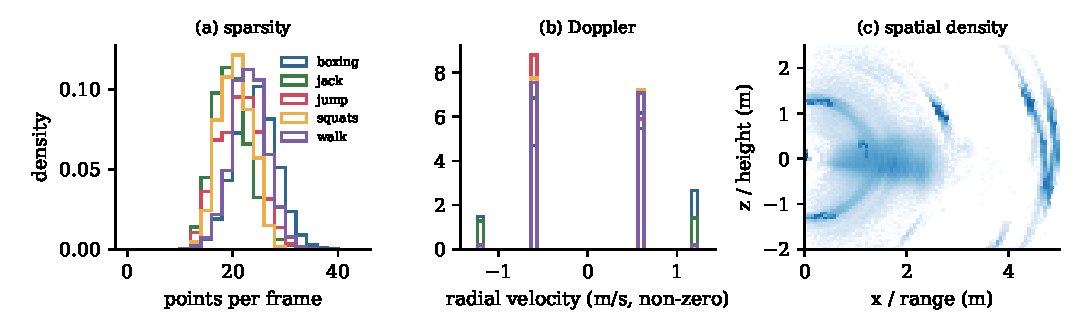
\includegraphics[width=\textwidth]{eda_radhar.pdf}
\caption{RadHAR. (a) points per frame by class; (b) non-zero Doppler values, which take only a few quantised values ($\pm0.6$, $\pm1.2$\,m/s); (c) density of all returns in the range--height plane (log scale): the person sits at 1--2\,m, and static clutter bands lie at about 2.5\,m and 4.5\,m.}
\label{fig:edarh}
\end{figure}

\begin{figure}[h]
\centering
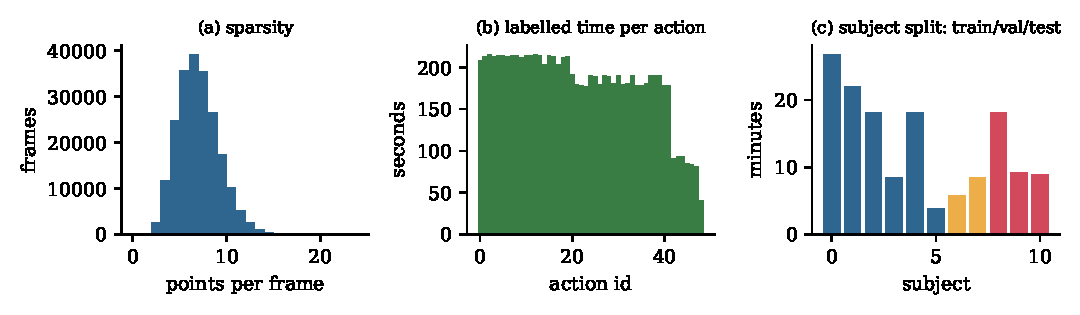
\includegraphics[width=\textwidth]{eda_milipoint.pdf}
\caption{MiliPoint. (a) points per frame (median 6); (b) labelled time per action; (c) labelled minutes per subject and the subject-disjoint split (blue train, orange validation, red test).}
\label{fig:edamp}
\end{figure}

\begin{figure}[h]
\centering
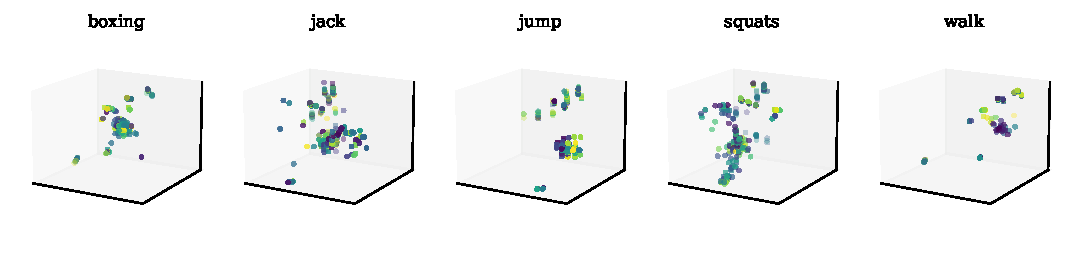
\includegraphics[width=\textwidth]{radhar_examples.pdf}
\caption{One pre-processed 2-s RadHAR test window per class (points coloured by time).}
\label{fig:rhex}
\end{figure}

\section{Class distribution}
RadHAR training recordings per class (boxing, jack, jump, squats, walk) are
26/28/26/29/33 and test recordings 13/10/11/10/14. The test windows per class
are 714/673/734/674/770, which is close to balanced. Some training recordings
are much longer than the standard 20\,s (for example \texttt{boxing\_184s.txt}
and \texttt{\_\_\_squats\_186s.txt}). This turned out to matter for validation
(Issue \#16--\#17). MiliPoint actions 0--40 have about 200\,s of labelled data
each, and actions 41--48 fewer (Fig.~\ref{fig:edamp}b).

\section{Noise characteristics (measured, not assumed)}
\begin{itemize}[nosep]
\item \textbf{Antenna self-returns}: 34.6\% of RadHAR returns lie at $x<0.3$\,m.
\item \textbf{Static clutter / multipath}: after the ROI filter, 50.1\% of returns lie more than
  1.2\,m (horizontally) from the moving-point centre of the person. They form
  persistent clusters at fixed ranges with zero Doppler (Fig.~\ref{fig:preprocreport}).
\item \textbf{Sparsity and variable density}: 15--28 returns per frame (5th--95th
  percentile) on RadHAR, and a median of 6 on MiliPoint.
\item \textbf{Doppler quantisation}: velocities take a handful of discrete values.
\item \textbf{Not observed}: corrupted files, NaN values or duplicated recordings
  (verified by the leakage audit, Chapter~\ref{ch:leak}).
\end{itemize}
Random coordinate displacement, point dropout, false detections and frame loss
are \emph{not} directly measurable without ground-truth body surfaces. They are
therefore studied as \emph{controlled synthetic perturbations} of recorded data
(Chapter~\ref{ch:pre}), and are clearly distinguished from the measured noise
above.

\section{Can the datasets be combined?}
Not as one training set. The label sets differ (5 vs 49 classes, and MiliPoint
action names are not published, so no reliable label mapping exists). The radars
differ (IWR1443 vs IWR1843), MiliPoint lacks Doppler and intensity, and the axes
differ. We therefore run \textbf{independent experiments} per dataset and use the
other dataset only for \textbf{representation transfer} after harmonising the
axes and restricting the input to $xyz$ (Chapter~\ref{ch:results}).

\section{Existing evaluation protocols}
RadHAR: an official train/test partition by recording, with validation on a
random 20\% of training \emph{windows} (which overlap by 50/60 frames).
MiliPoint: the published code concatenates labelled frames from all files and
cuts them chronologically 80/10/10, so the test data contain subjects that also
appear in training; other work uses random 80/10/10 splits \cite{zakka2025makgcn}.
Chapter~\ref{ch:leak} measures the leakage of each protocol.

\section{Dataset limitations}
RadHAR has no subject IDs and only two subjects. Its official test recordings were
made on the same days as the training recordings, often minutes apart
(Chapter~\ref{ch:leak}). MiliPoint provides $xyz$ only, and its action names are
unknown. Neither dataset contains falls or multi-person scenes.

\chapter{System Architecture and Design Decisions}

\section{Overall architecture}
Figure~\ref{fig:system} shows the complete system. Offline, raw dataset files are
parsed into per-recording frame arrays and cut into leakage-free splits. A data
module turns every 2-s window into a fixed tensor. The training script fits a
model and selects a checkpoint on validation data only. The analysis scripts
evaluate the held-out test set, the noise conditions and the statistics. The
exported model \emph{bundle} (weights + pre-processing settings + class names)
is the only artefact that the inference script and the demonstration
application need.

\begin{figure}[h]
\centering
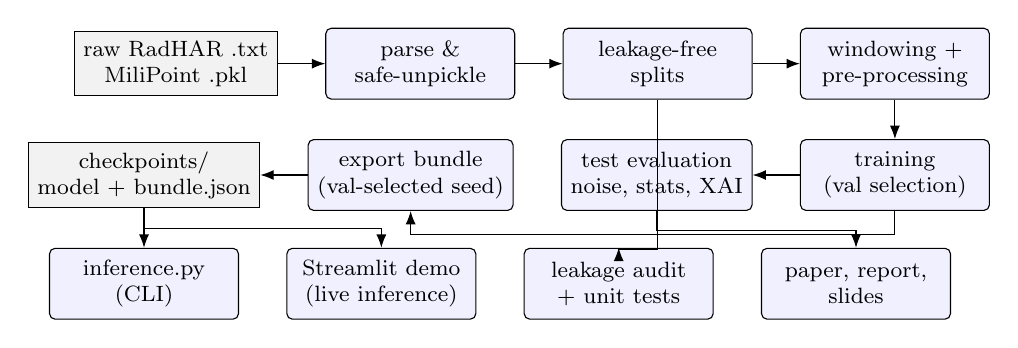
\begin{tikzpicture}[font=\footnotesize, >=Latex, node distance=5mm and 6mm,
  b/.style={draw, rounded corners=2pt, align=center, minimum height=9mm, minimum width=24mm, fill=blue!6},
  d/.style={draw, align=center, minimum height=8mm, minimum width=22mm, fill=gray!10}]
\node[d] (raw) {raw RadHAR .txt\\MiliPoint .pkl};
\node[b, right=of raw] (parse) {parse \&\\safe-unpickle};
\node[b, right=of parse] (split) {leakage-free\\splits};
\node[b, right=of split] (win) {windowing +\\pre-processing};
\node[b, below=of win] (train) {training\\(val selection)};
\node[b, left=of train] (eval) {test evaluation\\noise, stats, XAI};
\node[b, left=of eval] (export) {export bundle\\(val-selected seed)};
\node[d, left=of export] (bundle) {checkpoints/\\model + bundle.json};
\node[b, below=of bundle] (inf) {inference.py\\(CLI)};
\node[b, right=of inf] (app) {Streamlit demo\\(live inference)};
\node[b, right=of app] (audit) {leakage audit\\+ unit tests};
\node[b, right=of audit] (docs) {paper, report,\\slides};
\draw[->] (raw)--(parse); \draw[->] (parse)--(split); \draw[->] (split)--(win); \draw[->] (win)--(train);
\draw[->] (train)--(eval); \draw[->] (train.south) |- ++(0,-0.3) -| (export.south); \draw[->] (export)--(bundle);
\draw[->] (bundle)--(inf); \draw[->] (bundle.south) |- ++(0,-0.25) -| (app.north); \draw[->] (eval.south) |- ++(0,-0.25) -| (docs.north);
\draw[->] (split.south) |- ++(0,-1.9) -| (audit.north);
\end{tikzpicture}
\caption{End-to-end system architecture.}
\label{fig:system}
\end{figure}

\section{Components}
For each component, Table~\ref{tab:components} gives what it is, why it is used,
the alternatives considered, how it connects to the rest of the system, and its
limitations.

\begin{longtable}{L{2.2cm}L{3.3cm}L{3.0cm}L{3.0cm}L{3.0cm}}
\caption{Component design decisions.}\label{tab:components}\\
\toprule
Component & What / why & Alternatives & Connections & Limitations \\
\midrule\endfirsthead
\toprule Component & What / why & Alternatives & Connections & Limitations \\ \midrule\endhead
Parser (\texttt{radhar\_parse.py}) & regex over ROS text; frame = run of \texttt{point\_id} from 0. Needed because only raw dumps exist & the original voxel script (slow, keeps no Doppler) & produces \texttt{radhar\_frames.npy} for the data module and the demo & relies on the ROS dump format \\
Safe unpickler & loads MiliPoint pickles but allows only numpy reconstruction & plain \texttt{pickle.load} (allows code execution) & feeds \texttt{data\_milipoint.py} & a whitelist must be extended if the file format changes \\
Data module (\texttt{data\_radhar.py}) & windowing, ROI, person centring, gating, per-segment sampling, augmentation & voxel grids; fixed zero-padding & used by training, evaluation, inference and the demo, so pre-processing is identical everywhere & 2-s windows only \\
Models (\texttt{models.py}) & 7 architectures behind one interface \texttt{f(x, mask)} & PyG implementations & built by \texttt{build(name)}; used by training and inference & pure-PyTorch FPS/$k$-NN are slower than CUDA kernels \\
Training (\texttt{train.py}) & AdamW, one-cycle, label smoothing, early stopping on val macro-F1, optional KD / robust augmentation & SGD, fixed epochs & reads \texttt{configs/default.yaml}; writes run directories & CPU-bound \\
Noise (\texttt{noise.py}) & seeded perturbations for evaluation and training & ad-hoc numpy noise & robustness study, robust training, demo & synthetic, not physical radar simulation \\
Inference (\texttt{inference.py}) & loads a bundle and applies the training pre-processing to raw input & re-implementing pre-processing in the app & CLI and demo & needs at least 2\,s of data \\
Demo (\texttt{demo/app.py}) & interactive upload, visualisation, live prediction, noise injection & Gradio & imports \texttt{inference.py} & desktop browser; no live radar stream \\
Audit (\texttt{leakage\_audit.py}) & automated overlap/duplicate/statistics checks & manual inspection & reads splits and run logs & cannot detect subject overlap without subject IDs \\
\bottomrule
\end{longtable}

\section{Data-processing architecture}
Raw data $\rightarrow$ per-recording arrays (points, frame index, timestamps)
$\rightarrow$ recording/subject-level split $\rightarrow$ window list (recording, start
frame) $\rightarrow$ on-the-fly tensor construction. Building tensors on the fly
keeps memory small and lets each epoch draw different point samples, which acts as
augmentation.

\section{Training and inference architecture}
Training uses one process per configuration (one CPU thread) and a small job queue
(\texttt{scripts/runner.py}) that runs two jobs in parallel, skips finished jobs and
resolves dependencies (a distilled student waits for its teacher). Inference
runs one forward pass per 2-s window (sliding by 1/3\,s) and reports a
recording-level majority vote.

\section{Application architecture}
The Streamlit application caches the loaded bundle, validates the uploaded file,
calls \texttt{Bundle.windows\_from\_frames} (the same code path as evaluation) and
renders Plotly 3-D views. It is described in Chapter~\ref{ch:demo}.

\section{Edge deployment}
The proposed model has no data-dependent sampling (no FPS or $k$-NN), only dense
matrix products on tensors of fixed size ($12\times32$ points). This makes it
straightforward to export to ONNX or TFLite-Micro-style runtimes. Its INT8 weights
occupy \oursIntMB\,MB and one inference costs \oursMflops\,MFLOPs; the measured
single-thread CPU latency is \oursLat\,ms. Deployment on an actual micro-controller
was out of scope and has not been verified.

\section{Decision traceability matrix}
Table~\ref{tab:trace} links every important decision to the alternatives that
were investigated and to the evidence behind the final choice. ``Issue \#'' refers
to the development log (Chapter~10).

\begin{longtable}{L{2.0cm}L{3.2cm}L{2.6cm}L{3.4cm}L{3.0cm}}
\caption{Decision traceability matrix.}\label{tab:trace}\\
\toprule
Decision & Alternatives investigated & Final selection & Reason & Supporting evidence \\
\midrule\endfirsthead
\toprule Decision & Alternatives & Final & Reason & Evidence \\ \midrule\endhead
Dataset & MM-Fi, mmBody & MiliPoint (primary), RadHAR (secondary) & prescribed; public; subject IDs (MiliPoint); Doppler (RadHAR) & Ch.~3; licences BSD-3 / MIT \\
Combining datasets & joint training & separate experiments + $xyz$ transfer & label sets, sensors and features differ & Ch.~3 analysis; transfer results (Table~\ref{tab:transferreport}) \\
Input representation & voxel grids; single frames & 12 segments $\times$ 32 points, 2-s window & frames too sparse (6--21 pts); voxels mostly empty & EDA; voxel baseline results \\
Noise handling & DBSCAN; statistical/radius outlier removal; plain centroid & ROI + moving-point centring + 1.2\,m gating & clutter is static and far from the moving person & range histograms (Issue \#13); Fig.~\ref{fig:preprocreport}; gating ablation \\
Model architecture & PointNet, PointNet++, DGCNN, Point Transformer, voxel CNN-LSTM, PointNet-LSTM & STPT-Lite (+KD) & accuracy/efficiency trade-off under identical protocol & Tables~\ref{tab:radharreport}--\ref{tab:mpreport} \\
Compression & dynamic INT8; no compression & KD + weight-only INT8 & dynamic INT8 lost 7 pts and was slower & Issue \#11; INT8 accuracy in results \\
Data splitting & random windows (RadHAR original, some MiliPoint work); chronological & recording-disjoint (RadHAR), subject-disjoint (MiliPoint) & overlapping windows leak & leakage audit (Ch.~8) \\
Validation composition & all windows of each recording & $\leq$55 windows per recording & one long recording dominated selection & Issue \#16--\#17 \\
Optimiser & SGD; Adam & AdamW + one-cycle & standard for attention models; stable & training curves \\
Loss & plain cross-entropy; class weights & CE + label smoothing 0.1 (+KD) & near-duplicate windows; balanced classes & class counts (Ch.~3) \\
Regularisation & none / heavy augmentation & weight decay, dropout, early stopping, standard + optional robust augmentation & generalisation & augmentation ablation; robustness study \\
Model checkpoint & last epoch; best test & best validation macro-F1; exported seed chosen by validation & no test leakage in selection & audit: checkpoint consistency \\
Demo framework & Gradio, Flask & Streamlit + Plotly & interactive 3-D, built-in test harness & AppTest results (Ch.~13) \\
Point operations library & PyTorch Geometric, torch-cluster & pure PyTorch & no compiled extensions; portable & runs on CPU-only environment \\
\bottomrule
\end{longtable}

\chapter{Data Pre-processing and Noise Handling}
\label{ch:pre}

The pipeline (implemented in \texttt{src/data\_radhar.py}, shared by both
datasets) is described below, technique by technique, in the
\emph{what / why / how / effect / limitation / verification} format.

\begin{figure}[h]
\centering
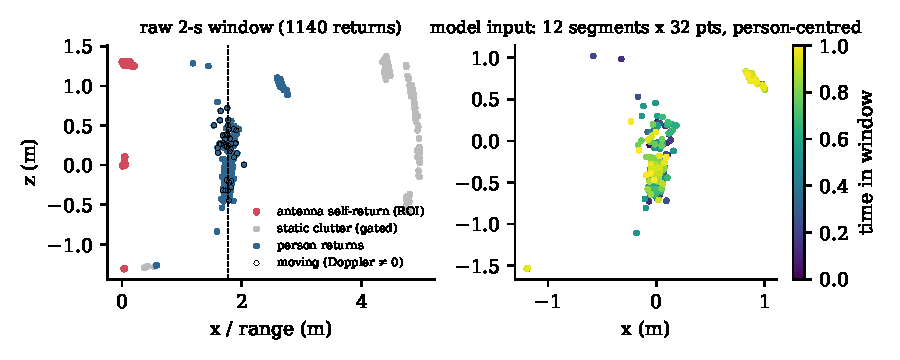
\includegraphics[width=\textwidth]{preproc_before_after.pdf}
\caption{One raw 2-s RadHAR window (left), with antenna self-returns (red),
static clutter removed by gating (grey), person returns (blue) and moving returns
(black circles), and the resulting model input (right).}
\label{fig:preprocreport}
\end{figure}

\section{Windowing}
\textbf{What:} 2-s windows (60 frames on RadHAR, 48 on MiliPoint) cut from one
recording or single-action run. \textbf{Why:} single frames hold only 6--21
returns and no motion information, and 2\,s matches the RadHAR protocol.
\textbf{How:} \texttt{make\_windows}; evaluation stride 10 frames (RadHAR) and 12
(MiliPoint); training stride 20 and 24, respectively. \textbf{Effect:} 3{,}565
RadHAR test windows (the original paper reports 3{,}538). \textbf{Limitation:}
activities shorter than 2\,s are not modelled. \textbf{Verification:} window
counts per split in the leakage audit.

\section{Region-of-interest (ROI) filter}
\textbf{What:} drop returns with $x<0.3$\,m (RadHAR only). \textbf{Why:} 34.6\% of
all returns are antenna self-reflections at $x\approx0$ (red points in
Fig.~\ref{fig:preprocreport}). \textbf{How:} \texttt{roi\_filter}. \textbf{Effect:}
these returns no longer distort the centroid or consume sampling slots.
\textbf{Limitation:} a person standing within 30\,cm of the radar would be
removed (an unrealistic set-up). \textbf{Verification:} EDA statistics.

\section{Person centring with moving returns}
\textbf{What:} express coordinates relative to the median of the window's
\emph{moving} returns (Doppler $\neq0$); fall back to the median of all returns.
\textbf{Why:} a plain centroid was pulled metres away by clutter (Issue \#13).
Static objects have zero radial velocity, whereas a performing person always
produces some moving returns. The median is robust to the remaining outliers.
\textbf{How:} \texttt{RadHARWindows.person\_centre}. \textbf{Effect:} translation
invariance with respect to where the person stands; removes distance as a cue.
\textbf{Limitation:} a motionless person has no moving returns (fallback used);
two moving people would be merged. \textbf{Verification:} ablation ``no centring''
was dropped for compute reasons. The gating ablation (below) covers the combined
effect.

\section{Spatial gating (clutter removal)}
\textbf{What:} drop returns more than 1.2\,m (horizontal distance) from the person
centre. \textbf{Why:} after the ROI filter, 50.1\% of returns are static clutter
clusters at 2.5\,m and 4.5\,m. Because training and test recordings share the
room, this clutter is also a potential scene \emph{shortcut}. \textbf{How:} applied
per segment before sampling. 1.2\,m covers arm span and in-place walking (the
median distance of returns from the centre is 0.9--1.6\,m before gating).
\textbf{Effect:} the sampled points come from the person. \textbf{Limitation:}
returns from limbs farther than 1.2\,m would be lost; the radius was chosen from
EDA, not tuned on test data. \textbf{Verification:} ablation \emph{-- spatial gating}
(Table~\ref{tab:ablation}).

\section{Temporal segmentation and point sampling}
\textbf{What:} split the window into $G=12$ segments and sample $P=32$ returns per
segment (with replacement if fewer). \textbf{Why:} a fixed tensor size is needed
for batching and edge inference; accumulating 4--5 frames per segment densifies
the cloud while keeping temporal order. \textbf{How:} \texttt{\_\_getitem\_\_};
evaluation uses a fixed per-sample seed so that test inputs are deterministic.
\textbf{Effect:} $12\times32\times6$ input. \textbf{Limitation:} duplicated points
when segments are sparse. \textbf{Verification:} unit test of shapes and
determinism.

\section{Feature normalisation}
Intensity is standardised with mean and standard deviation computed on the
\emph{training recordings only}. The validation and test sets reuse these values
(verified by the audit, Chapter~\ref{ch:leak}). Coordinates are already in
metres and person-centred. Time is normalised to $[0,1]$.

\section{Training-time augmentation}
\label{sec:aug}
\textbf{Standard (all models):} random rotation about the vertical axis
($\pm15^\circ$), isotropic scaling ($[0.9,1.1]$), 1-cm Gaussian jitter, and fresh
point sampling every epoch. \textbf{Noise-robust training (optional,
\texttt{--robust 1}):} per batch, each with probability 0.5: variable per-segment
density (keep 30--100\%), point dropout (0--20\%), false-detection injection
(0--10\% of returns), and with probability 0.25 the loss of one temporal segment.
All of these are applied to training batches only, from a separate random
generator (seeded $10{,}000+\mathrm{seed}$) that is never used at test time.

\section{Controlled noise conditions for evaluation}
Measured dataset noise (self-returns, clutter, sparsity) is handled by the
pre-processing above. To probe robustness beyond it, the \emph{test} inputs are
perturbed synthetically (\texttt{src/noise.py}), after pre-processing, with fixed
seeds so that every model sees identical perturbed samples
(Table~\ref{tab:noisecond}). These conditions are experimental manipulations,
not claims about the noise present in the datasets.

\begin{table}[h]
\centering
\caption{Evaluation perturbations (applied to the held-out test set only).}
\label{tab:noisecond}
\small
\begin{tabular}{L{2.6cm}L{6.2cm}L{4.6cm}}
\toprule
Condition & Operation & Levels \\
\midrule
Coordinate jitter & add $\mathcal{N}(0,\sigma^2)$ to $x,y,z$ & $\sigma=0.02, 0.05, 0.10$\,m \\
Point dropout & remove returns (slots masked, variable count) & 5, 15, 30\% \\
Increased sparsity & keep a fraction of unique returns, re-sample to $P$ & keep 50, 25, 12.5\% \\
Outlier injection & replace returns by uniform false detections in $\pm1.5$\,m & 5, 10, 20\% \\
Variable density & per-segment keep fraction $\sim U(k,1)$ & $k=0.5, 0.25, 0.1$ \\
Frame loss & drop whole temporal segments & 25, 50\% of segments \\
Combined & density + jitter + outliers + dropout & severity 1, 2, 3 \\
\bottomrule
\end{tabular}
\end{table}

\section{Methods investigated but not used}
Statistical and radius-based outlier removal and DBSCAN clustering were
considered. Gating around the moving-point centre removes the dominant clutter
with one interpretable parameter and no per-window clustering cost. Additional
filters on the remaining sparse body returns would risk removing limb points, so
they were not adopted. This decision was made from the EDA (the clutter forms
far-away clusters) and was not tuned on test data.

\chapter{Model Selection and Architecture}
\label{ch:model}

\section{Candidate architectures}
\textbf{PointNet} \cite{qi2017pointnet}: $f(\{\mathbf{p}_i\})=\gamma(\max_i h(\mathbf{p}_i))$,
where $h$ is a shared MLP and $\gamma$ a classifier. The max is permutation-invariant.
It is cheap, but no local geometry is modelled.
\textbf{PointNet++} \cite{qi2017pointnet2}: set-abstraction levels, each consisting
of FPS sampling of $n'$ centroids, a ball query (radius $r$, at most $k$
neighbours) and a PointNet on every local group.
\textbf{DGCNN} \cite{wang2019dgcnn}: EdgeConv
$\mathbf{h}_i'=\max_{j\in\mathcal{N}_k(i)}\phi(\mathbf{h}_j-\mathbf{h}_i,\mathbf{h}_i)$
over a $k$-NN graph that is recomputed in feature space at every layer.
\textbf{Point Transformer} \cite{zhao2021pt}: vector attention
$\mathbf{y}_i=\sum_{j\in\mathcal{N}_k(i)}\rho(\gamma(\varphi(\mathbf{x}_i)-\psi(\mathbf{x}_j)+\delta_{ij}))\odot(\alpha(\mathbf{x}_j)+\delta_{ij})$
with relative position encoding $\delta_{ij}=\theta(\mathbf{p}_i-\mathbf{p}_j)$.
\textbf{PointNet+BiLSTM}: a PointNet per temporal segment followed by a BiLSTM, as
in recent radar HAR work \cite{gu2024lpn}.
\textbf{Voxel TD-CNN+BiLSTM}: the RadHAR baseline \cite{singh2019radhar}.

\section{Selection rationale}
The brief names a lightweight point transformer as the primary direction,
provided the evidence supports it. Our design starts from the established parts,
namely Transformer self-attention \cite{vaswani2017attention}, relative-position
attention on points \cite{zhao2021pt} and PointNet-style pooling
\cite{qi2017pointnet}, and adapts them to the structure of the radar data:
\begin{enumerate}[nosep]
\item Sparse frames but strong temporal order $\Rightarrow$ attention is
  \emph{factorised}: first within short segments (spatial), then across segment
  tokens (temporal). This removes FPS and $k$-NN entirely.
\item Radar measures velocity $\Rightarrow$ an explicit per-segment motion
  descriptor is added to every token.
\item Edge cost $\Rightarrow$ width $d=64$, 2 temporal blocks, distillation from a
  wider teacher, INT8 weights.
\end{enumerate}
\textbf{Established vs.\ project-specific.} Multi-head self-attention, the
pre-norm Transformer block, the [CLS] token, attentive/max pooling, knowledge
distillation and per-channel weight quantisation are established techniques.
Project-specific are: the factorisation into intra-segment and inter-segment
attention for radar windows, the learned 3-D relative-position \emph{bias} inside
segments, the radar motion descriptor, and the moving-point centring and gating
pre-processing. Every project-specific component is ablated in
Table~\ref{tab:ablation}.

\section{Layer-by-layer architecture of STPT-Lite}
\begin{longtable}{L{3.6cm}L{3.0cm}L{3.0cm}L{4.6cm}r}
\caption{STPT-Lite layers (batch $B$, $G=12$, $P=32$, $d=64$, $H=4$ heads, $K$ classes). Parameter counts for $K=5$.}\label{tab:layers}\\
\toprule
Layer & Input & Output & Operation & Params \\
\midrule\endfirsthead
\toprule Layer & Input & Output & Operation & Params \\ \midrule\endhead
Point embedding & $B G P\times6$ & $BGP\times64$ & Linear--LN--GELU--Linear--LN--GELU & 4{,}864 \\
Intra-segment attention & $(BG)\times P\times64$ & same & pre-LN, QKV linear, softmax$(QK^\top/\sqrt{16}+\beta(\Delta\mathbf{p})+\log m)V$, output proj. & 16{,}768 \\
Relative-position bias $\beta$ & $P\times P\times3$ & $P\times P\times4$ & MLP $3\!\to\!16\!\to\!H$ & 132 \\
Feed-forward & $(BG)P\times64$ & same & LN, Linear $64\!\to\!128$, GELU, Linear $128\!\to\!64$, residual & 16{,}704 \\
Segment pooling & $(BG)\times P\times64$ & $(BG)\times64$ & attentive pool $\|$ masked max $\to$ Linear $128\!\to\!64$ & 8{,}321 \\
Motion descriptor & $B\times G\times8$ & $B\times G\times64$ & MLP $8\!\to\!32\!\to\!64$, added to tokens & 2{,}464 \\
{[CLS]} + positions & $B\times G\times64$ & $B\times13\times64$ & concatenate, add learned positions & 896 \\
Temporal block $\times2$ & $B\times13\times64$ & same & pre-LN MHSA ($H=4$, key padding mask) + FFN ($2d$) & 66{,}944 \\
Head & $B\times64$ & $B\times K$ & LN on [CLS], dropout 0.2, Linear & 453 \\
\midrule
Total & & & & 117{,}546 \\
\bottomrule
\end{longtable}

The motion descriptor of segment $g$ is
$\mathbf{u}_g=[\bar{\mathbf{x}}_g,\ \bar{\mathbf{x}}_g-\bar{\mathbf{x}}_{g-1},\ \overline{|v|}_g,\ \log(1+n_g)]$,
i.e.\ centroid (3), centroid displacement (3), mean absolute Doppler (1) and log
point count (1).

\section{Computational complexity}
Joint self-attention over all $N=GP=384$ points of a window costs
$O(N^2d)\approx9.4$\,M multiply-adds per layer. The factorised design costs
$O(GP^2d+G^2d)\approx0.8$\,M + 0.01\,M. Measured with PyTorch's FLOP counter, the
whole model needs \oursMflops\,MFLOPs per 2-s window. PointNet++, DGCNN and Point
Transformer additionally spend time on FPS loops and $k$-NN/ball queries, which
are sequential or $O(N^2)$ (Table~\ref{tab:radharreport}).

\section{Training variants and final model selection}
Three training variants of STPT-Lite were compared under identical settings:
plain training, knowledge distillation from STPT-Large (KD), and KD combined with
noise-robust augmentation (Section~\ref{sec:aug}; \texttt{src/noise.py:robust\_augment}:
per batch, with probability 0.5 each, variable density with minimum keep 0.3,
dropout up to 20\%, false detections up to 10\%, and with probability 0.25 the
loss of one segment). Jitter and extreme sparsity are not used in training, so they
remain unseen corruption types at test time. The final model was selected on
\emph{validation} macro-F1 averaged over seeds on both datasets (Issue~\#39):
KD+robust had the highest mean validation macro-F1 on RadHAR and on MiliPoint, and
it is the model that is exported, served by the demo and reported as ``proposed''.
Test accuracy was not used for this choice.

\section{Variants}
\begin{table}[h]
\centering
\caption{Model variants used in the experiments (parameters for 5 / 49 classes).}
\label{tab:variants}
\small
\begin{tabular}{L{3.4cm}L{6.4cm}r r}
\toprule
Model & Configuration & Params (5) & Params (49) \\
\midrule
STPT-Large (teacher) & $d=128$, 4 temporal blocks, 8 heads & 725{,}262 & 730{,}938 \\
STPT-Lite (proposed) & $d=64$, 2 blocks, 4 heads & 117{,}546 & 120{,}406 \\
STPT-Tiny & $d=32$, 2 blocks, 4 heads & 30{,}682 & 32{,}134 \\
PointNet & MLP 64-128-256, max-pool & 76{,}229 & 81{,}905 \\
PointNet+BiLSTM & per-segment PointNet 64-128, BiLSTM 64 & 109{,}125 & 114{,}801 \\
PointNet++ (SSG) & SA(128, 0.3\,m, 16) -- SA(32, 0.6\,m, 16) -- global & 413{,}381 & 424{,}689 \\
DGCNN & 3 EdgeConv ($k=16$), 128 points & 422{,}405 & 433{,}713 \\
Point Transformer & 2 PT blocks + transition down, 128 points & 335{,}237 & 340{,}913 \\
Voxel TD-CNN+BiLSTM & $10\times32\times32$ voxels, 3-D conv 8/16/16, BiLSTM 16 & 45{,}861 & 47{,}313 \\
\bottomrule
\end{tabular}
\end{table}

\chapter{Training and Optimisation}

\section{Environment}
\label{sec:env}
\begin{table}[h]
\centering
\caption{Computational environment.}
\label{tab:env}
\small
\begin{tabular}{L{4cm}L{10cm}}
\toprule
Hardware & 2 vCPU (Intel Xeon), 7\,GB RAM, no GPU (Linux cloud workspace) \\
Software & Python 3.13, PyTorch 2.15, NumPy 2.5, scikit-learn 1.9, SciPy 1.18, pandas 3.0, Matplotlib 3.11, Streamlit 1.67, Plotly 7.1 \\
Parallelism & 2 training jobs in parallel, 1 thread each (\texttt{scripts/runner.py}) \\
Latency measurement & batch 1, single thread, median of 200 runs after 20 warm-up runs \\
\bottomrule
\end{tabular}
\end{table}

\section{Hyper-parameters and their justification}
All hyper-parameters are in \texttt{configs/default.yaml}. They were fixed
\emph{before} any test-set evaluation and are identical for every model, so the
comparison is fair. Table~\ref{tab:hp} lists them.

\begin{longtable}{L{3.2cm}L{3.2cm}L{8.0cm}}
\caption{Training configuration.}\label{tab:hp}\\
\toprule
Setting & Value & Reason \\
\midrule\endfirsthead
\toprule Setting & Value & Reason \\ \midrule\endhead
Optimiser & AdamW \cite{loshchilov2019adamw} & decoupled weight decay is the standard for Transformers; robust default for all models \\
Learning rate & $2\times10^{-3}$ peak & small models and batch 64; converged within a few epochs in smoke tests \\
Schedule & one-cycle, 10\% warm-up & warm-up stabilises attention early; annealing to near zero gives a well-defined end point \\
Weight decay & 0.05 & regularisation for a small dataset \\
Batch size & 64 & CPU throughput vs.\ gradient noise \\
Loss & cross-entropy, label smoothing 0.1 \cite{szegedy2016inception} & avoids over-confident outputs on near-duplicate windows \\
Class weights & none & classes are nearly balanced (Chapter~\ref{ch:data}) \\
Dropout & 0.1 (attention/FFN), 0.2--0.5 (heads) & standard values for each architecture \\
Gradient clipping & global norm 1.0 & prevents rare spikes from the attention softmax \\
Max epochs & 15 & upper bound only \\
Early stopping & patience 5 on validation macro-F1 & stop when the model no longer generalises better \\
Checkpoint & best validation macro-F1 & model selection on validation data only \\
KD & $\alpha=0.7$, $T=4$ \cite{hinton2015kd} & common values; teacher = STPT-Large trained with the same seed \\
Seeds & 0, 1, 2 & three independent runs; mean $\pm$ sample std reported \\
\bottomrule
\end{longtable}

\section{Overfitting prevention}
\begin{enumerate}[nosep]
\item Early stopping and best-checkpoint saving on validation macro-F1.
\item One-cycle learning-rate scheduling.
\item Regularisation: weight decay, dropout, label smoothing.
\item Training-only augmentation (Chapter~\ref{ch:pre}); validation and test inputs are deterministic.
\item Validation split by \emph{recording} (RadHAR) or \emph{subject} (MiliPoint), so selection
  reflects generalisation to unseen recordings or people.
\item Small models: the proposed model has 117.5\,K parameters, compared with 4{,}773 RadHAR
  training windows and about 4{,}500 MiliPoint training windows.
\end{enumerate}
For every epoch we log training loss, training accuracy, validation loss (NLL),
validation accuracy, validation macro-F1 and the learning rate
(\texttt{history.csv} in every run directory). The curves are discussed in
Chapter~\ref{ch:results}.

\section{Training-stability investigation}
In the first round of RadHAR runs, results varied strongly across seeds
(teacher: 95.5 / 96.1 / 87.0\%) and the distilled student selected its epoch-1
checkpoint. The investigation (Issue \#16--\#17) traced this to validation
composition. One 186-s squat recording contributed 553 of 2{,}709 validation
windows (20\%) and was predicted as ``jump'' throughout, so validation macro-F1
was dominated by a single recording. After capping each validation recording at 55
windows, validation and test accuracy agree (e.g.\ 94.5\% validation accuracy at
epoch 9 of the first re-run teacher). This is a genuine stability fix, not a
tuning of results: the test set was not used to make it.

\chapter{Data Leakage Prevention}
\label{ch:leak}

\section{Splitting methodology}
\textbf{RadHAR}: the official test recordings (58) are kept unchanged. The
remaining 142 training recordings are split 80/20 \emph{per class by recording}
(113 train, 29 validation, fixed seed 0, independent of the model seed).
\textbf{MiliPoint (primary)}: subject-disjoint, with subjects 8, 9, 10 for test,
subjects 6, 7 for validation, and the remaining six subjects for training. Windows
never cross the boundary of a single-action run.
\textbf{Comparison protocols} (MiliPoint only, never used for model development):
the chronological 80/10/10 cut of the MiliPoint code, and a random 80/10/10
split of overlapping windows.

\section{Restrictions}
\begin{itemize}[nosep]
\item \textbf{Pre-processing}: the only data-dependent statistic, the intensity
  mean and standard deviation, is computed on training recordings and reused
  unchanged for validation and test. Gating radius and ROI threshold come from the
  EDA and are not learned.
\item \textbf{Augmentation}: stochastic augmentation and robust-noise
  augmentation are applied only in training mode, from a separate random stream.
  Evaluation samples are deterministic (fixed per-index seed).
\item \textbf{Test-set protection}: the checkpoint is chosen by validation
  macro-F1. The test split is evaluated once per run, after training. No
  hyper-parameter, pre-processing threshold or architecture choice was changed in
  response to a test score. The only data-handling change made after the first
  runs, the validation cap, was motivated by validation behaviour (Issue \#17).
\item \textbf{Exported model}: the seed exported for the demo is chosen by
  validation macro-F1, not by test accuracy.
\end{itemize}

\section{Automated audit}
\texttt{scripts/leakage\_audit.py} recomputes every check from the data and run
files. Its output (\texttt{docs/leakage\_audit.md}) is reproduced in
Table~\ref{tab:audit}.

\begin{longtable}{L{4.6cm}L{6.6cm}L{2.8cm}}
\caption{Automated leakage-audit results.}\label{tab:audit}\\
\toprule
Check & Result & Status \\
\midrule\endfirsthead
\toprule Check & Result & Status \\ \midrule\endhead
\csname @@input\endcsname ../paper/generated/audit_rows.tex 
\bottomrule
\end{longtable}

\section{Findings}
\begin{enumerate}[nosep]
\item RadHAR splits share no recording, no identical recording content and no
  identical frame. Our splits are therefore recording-disjoint.
\item \textbf{RadHAR's official test set is not session-independent.} The ROS
  timestamps show that every test recording was made within 10 minutes of a
  training recording, on the same four days (median gap 29\,s), and the dataset
  provides no subject IDs. Subject-independent generalisation therefore
  \emph{cannot be verified} on RadHAR, and RadHAR accuracy should be read as
  ``new recordings, same people and room''.
\item On MiliPoint, the subject-disjoint split shares no subject and no frame
  between splits. This is the protocol that tests generalisation to new people,
  and it is our primary result.
\item The chronological protocol of the MiliPoint code shares subjects (0 and 8)
  between training and test.
\item The random-window protocol places \mpAuditLeakFrames\% of test frames inside
  training windows, and \mpAuditLeakWins\% of test windows overlap a training
  window (by \mpAuditLeakOverlap\% of the window on average). Accuracies obtained
  this way measure memorisation of near-duplicates; Chapter~\ref{ch:results}
  quantifies the inflation.
\item All completed runs satisfy ``saved checkpoint = epoch of maximal validation
  macro-F1'' (\auditSelConsistent{} of \auditSelRuns{} runs).
\end{enumerate}

\chapter{Implementation Details}

\section{Repository structure}
\begin{lstlisting}[numbers=none]
src/            radhar_parse.py  safe_pickle.py  data_radhar.py  data_milipoint.py
                models.py  noise.py  train.py  inference.py
configs/        default.yaml
scripts/        runner.py  jobs_main.txt  eda.py  analyze.py  xai_robust.py
                leakage_audit.py  export_model.py  make_numbers.py  run_all.sh
checkpoints/    exported inference bundles (model.pt, bundle.json, metrics.json)
demo/           app.py  samples/ (held-out test recordings)
tests/          test_pipeline.py (pytest)
results/        runs/<tag>/ (metrics.json, history.csv, probabilities, model.pt), summaries
docs/           DEVLOG.md  leakage_audit.md
paper/  report/ figures/
\end{lstlisting}

\section{Module descriptions}
\begin{longtable}{L{2.6cm}L{3.4cm}L{2.6cm}L{2.6cm}L{3.2cm}}
\caption{Modules: purpose, interfaces, error handling and verification.}\label{tab:modules}\\
\toprule
Module & Purpose / key functions & Input & Output & Errors / verification \\
\midrule\endfirsthead
\toprule Module & Purpose / key functions & Input & Output & Errors / verification \\ \midrule\endhead
\texttt{radhar\_parse} & \texttt{parse\_text}: regex over ROS messages; frames from \texttt{point\_id} resets & raw text & points $[N,5]$, frame $[N]$, timestamps & \texttt{ValueError} if no records; unit tests \\
\texttt{safe\_pickle} & restricted \texttt{Unpickler.find\_class} & .pkl path & Python objects & \texttt{UnpicklingError} for any non-numpy global; unit test with a malicious pickle \\
\texttt{data\_radhar} & \texttt{split\_recordings}, \texttt{make\_windows}, \texttt{RadHARWindows} (ROI, centring, gating, sampling, augmentation) & recordings dict & tensors $x[G,P,6]$, mask, label & shape/determinism tests; audit \\
\texttt{data\_milipoint} & run construction, axis remap, 3 split protocols & pkl files, \texttt{id.json} & same as above & subject-disjoint test; audit \\
\texttt{models} & 9 model classes; \texttt{build}, \texttt{n\_params} & $x$, mask & logits $[B,K]$ & forward test with empty segments for every model \\
\texttt{noise} & 7 seeded perturbations; \texttt{robust\_augment} & $x$, mask, generator & new $x$, mask & determinism, no in-place change, effect-size tests \\
\texttt{train} & training loop, KD, early stopping, metrics, INT8, FLOPs, latency & CLI + YAML & run directory & smoke runs; audit of checkpoint selection \\
\texttt{inference} & \texttt{Bundle}: load, pre-process raw input, predict, predict with noise & bundle dir, raw file & probabilities, latency & rejects short/NaN/wrong-shape input; tests \\
\texttt{demo/app.py} & Streamlit UI & bundle, upload/sample & interactive views & invalid uploads shown as errors; AppTest \\
\bottomrule
\end{longtable}

\section{Key code}
Factorised attention, segment tokenizer (\texttt{src/models.py}):
\begin{lstlisting}[language=Python]
f = self.emb(x)                                         # [N=B*G, P, d]
q, k, v = self.qkv(self.n1(f)).view(N, P, 3, h, d//h).permute(2, 0, 3, 1, 4)
bias = self.rel(x[:, :, None, :3] - x[:, None, :, :3]).permute(0, 3, 1, 2)
a = (q @ k.transpose(-1, -2)) / math.sqrt(d // h) + bias
a = a.masked_fill(m[:, None, None, :] == 0, -1e4).softmax(-1)
f = f + self.proj((a @ v).transpose(1, 2).reshape(N, P, d))
f = f + self.ff(self.n2(f))
\end{lstlisting}
Person centring and gating (\texttt{src/data\_radhar.py}):
\begin{lstlisting}[language=Python]
mov = allp[np.abs(allp[:, 3]) > 0]                      # moving returns (Doppler != 0)
ctr = np.median(mov[:, :3] if len(mov) else allp[:, :3], 0)
keep = np.linalg.norm(p[:, :2] - ctr[:2], axis=1) <= self.gate
\end{lstlisting}
Knowledge-distillation loss (\texttt{src/train.py}):
\begin{lstlisting}[language=Python]
kd = F.kl_div(F.log_softmax(logits / T, -1), F.softmax(tlog / T, -1),
              reduction='batchmean') * T ** 2
loss = (1 - alpha) * ce + alpha * kd
\end{lstlisting}

\section{Reproducibility}
Every run fixes \texttt{torch.manual\_seed}, NumPy's seed and the data-loader
generator. Evaluation inputs use a per-index seed. Each \texttt{metrics.json}
stores the full argument list, the YAML configuration and the PyTorch version.
\texttt{scripts/run\_all.sh} reproduces the full pipeline end to end.

\chapter{Failed Experiments, Errors and Rectification History}

This chapter reproduces the continuous issue-resolution log
(\texttt{docs/DEVLOG.md}). Entries are taken from the actual commands, error
messages, logs and results of the development; no entry was invented. Times are
UTC on 11 November 2026.

{\footnotesize
\setlength{\tabcolsep}{3pt}
\begin{longtable}{@{}r L{1.5cm}L{3.0cm}L{3.0cm}L{3.0cm}L{2.4cm}L{2.0cm}@{}}
\caption{Issue-resolution log.}\label{tab:devlog}\\
\toprule
\# & Stage & Issue / decision & Root cause / evidence & Correction & Verification & Outcome \\
\midrule\endfirsthead
\toprule \# & Stage & Issue / decision & Root cause / evidence & Correction & Verification & Outcome \\ \midrule\endhead
\csname @@input\endcsname ../paper/generated/devlog_rows.tex 
\bottomrule
\end{longtable}}

\section{Most consequential issues}
\textbf{Clutter-biased centring (\#13).} Symptom: in the exploratory plots, the
``centred'' model input placed the person about 0.7\,m off-centre, together with
a large second cluster. Diagnosis: range histograms of all returns vs.\ moving
returns showed that static clusters at 2.5\,m and 4.5\,m carried about half of
the returns, while all moving returns were on the person. Alternatives
considered: DBSCAN clustering (per-window cost, parameter sensitivity) and
radius/statistical outlier removal (removes sparse limb returns). Correction:
centring on moving returns plus 1.2\,m gating. Verification: the
before/after figure and the ablation \emph{-- spatial gating}. All runs were
restarted so that every reported number uses the same pipeline.

\textbf{Validation dominated by one recording (\#16--\#17).} Symptom: validation
accuracy (79\%) far below test accuracy (96\%), a seed spread of 9 points and an
epoch-1 checkpoint for one model. Diagnosis: per-recording validation accuracy
showed a single 186-s squat recording (20\% of validation windows) predicted as
``jump''. Correction: at most 55 evenly spaced windows per validation recording.
Verification: validation and test accuracy now agree. The test set played no
part in the fix.

\textbf{Quantisation (\#11).} PyTorch dynamic INT8 quantisation lost 7 points of
accuracy and was \emph{slower} for these tiny layers. Weight-only per-channel
INT8 kept accuracy (within 0.05 points) and reduced storage by a factor of 3.6.
Only the INT8 storage size is claimed, not an INT8 speed-up.

\textbf{Leakage findings (\#24--\#26).} The audit did not reveal leakage in our
own protocols. It did reveal that the RadHAR benchmark cannot test session or
subject independence, and that the random-window protocol used in some prior work
leaks most of its test frames into training. This changed the emphasis of the
evaluation (MiliPoint subject-disjoint as the primary result) and became a
contribution of the paper.

\chapter{Experimental Results}
\label{ch:results}

All numbers in this chapter are generated by \texttt{scripts/analyze.py} and
\texttt{scripts/make\_numbers.py} from the run directories, so they cannot drift
from the logs. Means and standard deviations are over the seeds stated in each
table. The test sets were evaluated once per run, with the checkpoint chosen on
validation data.

\section{Main comparison}
\begin{table}[h]
\centering
\caption{RadHAR official test recordings (3{,}565 windows, 5 classes). Mean\,$\pm$\,std over 3 seeds. Sig.: number of seeds in which the Holm-corrected McNemar test against the proposed model gives $p<0.05$; $\uparrow$ ours better / $\downarrow$ ours worse. Latency: median, batch 1, one CPU thread.}
\label{tab:radharreport}
\setlength{\tabcolsep}{5pt}
\resizebox{\textwidth}{!}{\begin{tabular}{lrrrccc}
\toprule
Model & Params (K) & MFLOPs & Lat. (ms) & Accuracy (\%) & Macro-F1 (\%) & Sig. \\
\midrule
Voxel TD-CNN+BiLSTM [RadHAR] & 45.9 & 180.5 & 6.60 & 95.01\,$\pm$\,0.16 & 95.03\,$\pm$\,0.17 & 2/3$\uparrow$ \\
PointNet & 76.2 & 31.8 & 0.74 & 96.31\,$\pm$\,0.66 & 96.36\,$\pm$\,0.64 & 1/3$\uparrow$ \\
PointNet+BiLSTM & 109.1 & 6.6 & 0.83 & 96.14\,$\pm$\,0.23 & 96.16\,$\pm$\,0.21 & 2/3$\uparrow$ \\
PointNet++ (SSG) & 413.4 & 133.1 & 8.44 & 97.34\,$\pm$\,0.18 & 97.37\,$\pm$\,0.19 & 1/3$\downarrow$ \\
DGCNN & 422.4 & 137.9 & 6.95 & 95.85\,$\pm$\,0.00 & 95.89\,$\pm$\,0.00 & 1/3$\uparrow$ \\
Point Transformer & 335.2 & 264.4 & 7.98 & 97.01\,$\pm$\,0.25 & 97.04\,$\pm$\,0.24 & 1/3$\uparrow$ \\
\midrule
STPT-Large (teacher) & 725.3 & 139.5 & 3.59 & 96.44\,$\pm$\,1.43 & 96.48\,$\pm$\,1.42 & 1/3$\uparrow$ \\
STPT-Lite & 117.5 & 36.6 & 2.14 & 96.22\,$\pm$\,1.43 & 96.27\,$\pm$\,1.41 & 2/3$\uparrow$ \\
STPT-Lite + KD & 117.5 & 36.6 & 2.08 & 96.04\,$\pm$\,0.78 & 96.08\,$\pm$\,0.76 & 1/3$\uparrow$ \\
STPT-Tiny + KD & 30.7 & 12.1 & 1.92 & 96.86\,$\pm$\,0.17 & 96.90\,$\pm$\,0.16 & 1/3$\uparrow$ \\
\textbf{STPT-Lite + KD + robust (ours)} & 117.5 & 36.6 & 2.58 & 96.83\,$\pm$\,0.69 & 96.88\,$\pm$\,0.68 & -- \\
PointNet + noise-robust training & 76.2 & 31.8 & 0.73 & \textbf{97.38\,$\pm$\,0.11} & \textbf{97.40\,$\pm$\,0.11} & 1/3$\downarrow$ \\
\bottomrule
\end{tabular}}
\end{table}
\begin{table}[h]
\centering
\caption{MiliPoint, subject-disjoint test (subjects 8--10, 3{,}569 windows, 49 actions). Same conventions as Table~\ref{tab:radharreport}.}
\label{tab:mpreport}
\setlength{\tabcolsep}{5pt}
\resizebox{\textwidth}{!}{\begin{tabular}{lrrrccrc}
\toprule
Model & Params (K) & MFLOPs & Lat. (ms) & Accuracy (\%) & Macro-F1 (\%) & Top-3 & Sig. \\
\midrule
PointNet & 81.9 & 31.8 & 0.74 & 32.57\,$\pm$\,4.59 & 29.72\,$\pm$\,4.50 & 59.5 & 3/3$\uparrow$ \\
PointNet+BiLSTM & 114.8 & 6.6 & 0.74 & 28.11\,$\pm$\,4.06 & 28.09\,$\pm$\,4.66 & 56.1 & 3/3$\uparrow$ \\
PointNet++ (SSG) & 424.7 & 133.1 & 7.94 & 8.07\,$\pm$\,5.47 & 5.12\,$\pm$\,5.76 & 21.4 & 3/3$\uparrow$ \\
STPT-Large (teacher) & 730.9 & 139.5 & 3.65 & \textbf{50.39\,$\pm$\,1.39} & \textbf{50.84\,$\pm$\,2.11} & 75.8 & 1/3$\uparrow$ \\
STPT-Lite & 120.4 & 36.6 & 2.60 & 45.79\,$\pm$\,6.30 & 45.95\,$\pm$\,7.05 & 73.9 & 1/3$\uparrow$ \\
STPT-Lite + KD & 120.4 & 36.6 & 2.07 & 48.55\,$\pm$\,4.35 & 47.62\,$\pm$\,6.08 & 76.4 & 1/3$\downarrow$ \\
\textbf{STPT-Lite + KD + robust (ours)} & 120.4 & 36.6 & 2.00 & 49.56\,$\pm$\,1.98 & 48.80\,$\pm$\,1.68 & 78.0 & -- \\
PointNet + noise-robust training & 81.9 & 31.8 & 0.78 & 18.66\,$\pm$\,8.83 & 15.67\,$\pm$\,8.98 & 40.9 & 3/3$\uparrow$ \\
\bottomrule
\end{tabular}}
\end{table}

\textbf{MiliPoint, unseen subjects (Table~\ref{tab:mpreport}).} The
STPT family clearly outperforms all re-implemented baselines.
The proposed STPT-Lite+KD+robust (selected on validation macro-F1, Issue~\#39)
reaches \mistptlitekdrobustAcc\,$\pm$\,\mistptlitekdrobustStd\% top-1
(\mistptlitekdrobustTopthree\% top-3); distillation alone gives
\mistptlitekdAcc\,$\pm$\,\mistptlitekdStd\%. This compares with \mipointnetAcc\,$\pm$\,\mipointnetStd\% for
the best baseline (PointNet). Every pairwise difference to a baseline is
significant in all three seeds (exact McNemar, Holm-corrected, $p<10^{-45}$).
Distillation raised the mean and, above all, removed a failed seed (STPT-Lite
without KD: one seed at 38.6\%).

\textbf{RadHAR (Table~\ref{tab:radharreport}).} All point-based models lie
between about 96 and 98\%, and differences between them are mostly within one
standard deviation. The proposed model reaches \rastptlitekdrobustAcc\,$\pm$\,\rastptlitekdrobustStd\%.
PointNet++ is the most accurate here, at 4--5$\times$ our
latency and 3.5$\times$ our parameter count. Every model, including the voxel
CNN-LSTM from the original paper, exceeds the published 90.47\%, which shows
the effect of the shared pre-processing.

\section{Per-class results and confusion}
\begin{figure}[h]
\centering
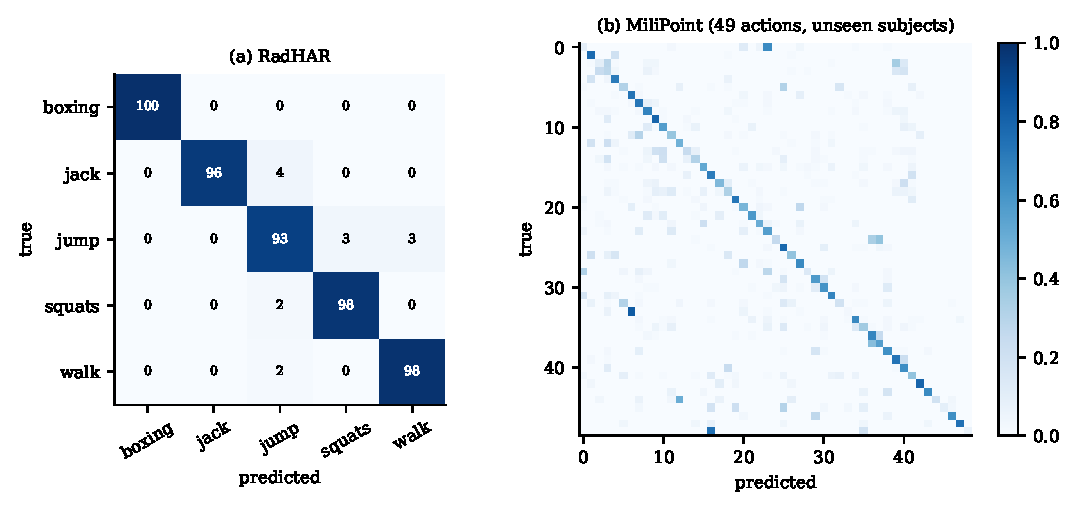
\includegraphics[width=\textwidth]{confusion.pdf}
\caption{Row-normalised confusion matrices of the proposed STPT-Lite+KD+robust (seed 0).}
\label{fig:confreport}
\end{figure}
\begin{table}[h]
\centering
\caption{Per-class test precision, recall and F1 (\%) of the proposed model (STPT-Lite+KD+robust) on RadHAR (mean over seeds).}
\label{tab:perclass}
\begin{tabular}{lrrrr}
\toprule
Class & Precision & Recall & F1 & Windows \\
\midrule
boxing & 99.86 & 99.91 & 99.88 & 714 \\
jumping jacks & 99.69 & 95.15 & 97.36 & 673 \\
jump & 91.01 & 94.41 & 92.66 & 734 \\
squats & 97.57 & 96.79 & 97.17 & 674 \\
walk & 96.83 & 97.79 & 97.31 & 770 \\
\bottomrule
\end{tabular}
\end{table}
On MiliPoint the per-action recall of the proposed model (mean over seeds) ranges from 6.4\% (action 33) to 83.9\% (action 9); 27 of 49 actions are recalled at $\geq$50\% and 6 below 20\%. The weakest actions are confused with kinematically similar ones (off-diagonal clusters in Fig.~\ref{fig:confreport}).

\section{Training and validation behaviour}
\begin{figure}[h]
\centering
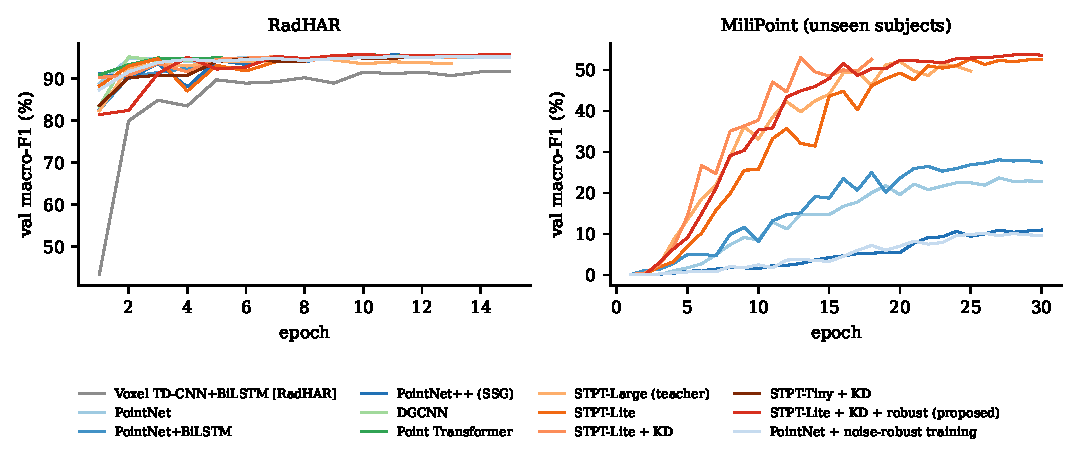
\includegraphics[width=\textwidth]{curves.pdf}
\caption{Validation macro-F1 per epoch (seed 0) for every model. RadHAR saturates within a few epochs; on MiliPoint the STPT models converge between epochs 15 and 30, while the PointNet family keeps a large gap.}
\label{fig:curvesreport}
\end{figure}
Training/validation loss, accuracy and learning rate for every epoch of every run
are stored in \texttt{results/runs/*/history.csv}. On RadHAR, 22 of 24 runs of the
cheaper models stopped early or peaked before the 15-epoch cap. On MiliPoint the
30-epoch cap was introduced after the first runs peaked at the 15-epoch cap
(Issue \#33). After the change, the STPT runs peaked between epochs 13 and 29.

\section{Ablation, protocol study and transfer}
\begin{table}[t]
\centering
\caption{Ablation of STPT-Lite (no distillation): test accuracy (\%), mean\,$\pm$\,std over seeds (variants: 2 on RadHAR, 2 on MiliPoint; full model: 3), change w.r.t.\ the full model trained with the same seeds in brackets; $^\dagger$ single run.}
\label{tab:ablation}
\setlength{\tabcolsep}{3pt}
\resizebox{\columnwidth}{!}{%
\begin{tabular}{lcc}
\toprule
Variant & RadHAR & MiliPoint (subj.) \\
\midrule
STPT-Lite (full, no KD) & 96.22\,$\pm$\,1.43 & 45.79\,$\pm$\,6.30 \\
\midrule
-- intra-segment attention (max+attentive pool only) & 96.90\,$\pm$\,0.18 (+0.93) & 42.87\,$\pm$\,3.03 (-6.52) \\
-- motion descriptor & 97.67\,$\pm$\,0.16 (+1.70) & 49.90\,$\pm$\,2.06 (+0.50) \\
-- temporal Transformer (mean over segments) & 96.70\,$\pm$\,0.61 (+0.73) & 37.54\,$\pm$\,6.62 (-11.85) \\
-- Doppler \& intensity ($xyz$ only) & 96.42\,$\pm$\,1.69 (+0.45) & -- \\
-- spatial gating & 97.62\,$\pm$\,0.40 (+1.64) & -- \\
-- all training augmentation & 96.68\,$\pm$\,0.54 (+0.70) & -- \\
-- coordinate jitter augmentation & 95.86\,$\pm$\,1.13 (-0.11) & -- \\
\bottomrule
\end{tabular}}
\end{table}
\textbf{MiliPoint (unseen people)} is the informative benchmark for the
architecture. Compared with the full model trained with the same two seeds
(49.4\% on average), removing the temporal Transformer (mean over segment
tokens instead) costs 11.9 points, and removing the intra-segment attention
(pooling only) costs 6.5 points. Both losses hold in each seed separately.
Fine-grained actions are therefore distinguished both by how the returns of a
short segment relate to each other and by how the segments evolve over the
window. The explicit motion descriptor brings no measurable gain (+0.5 points on
average, +2.8 and $-$1.8 in the two seeds): the attention layers apparently
recover centroid and displacement information from the point coordinates
themselves. We keep the descriptor because it costs only 2.5\,K parameters (2\% of the model), but
we do not claim it as a contribution to accuracy. \textbf{RadHAR} cannot rank
components. Every variant, including removing Doppler/intensity, gating or
augmentation, lies within about 1.7 points of the full model, inside its
seed spread ($\pm$1.4), because every model already exceeds 95\%. The
effect of the pre-processing is visible across models instead: with the same gating
and centring, all baselines exceed the published 90.47\%.


\begin{table}[t]
\centering
\caption{MiliPoint (49 actions) top-1 accuracy (\%) of the same models under three splits. Published numbers: 34.45 (PointNet++, \cite{cui2023milipoint}) and 98.25 (MAK-GCN, random 80/10/10, \cite{zakka2025makgcn}).}
\label{tab:protocol}
\setlength{\tabcolsep}{3pt}
\resizebox{\columnwidth}{!}{%
\begin{tabular}{lccc}
\toprule
Model & Subject-disjoint & Chronological & Random windows \\
 & (ours, primary) & (MiliPoint code) & (leaky) \\
\midrule
STPT-Lite & 45.79\,$\pm$\,6.30 & 58.38 (n=1) & 79.48 (n=1) \\
PointNet & 32.57\,$\pm$\,4.59 & 32.42 (n=1) & 44.44 (n=1) \\
\bottomrule
\end{tabular}}
\end{table}
\begin{table}[t]
\centering
\caption{Cross-dataset transfer (STPT-Lite, $xyz$ input): test accuracy (\%) when fine-tuning on a fraction of target training recordings/runs, from scratch vs.\ initialised from the model trained on the other dataset (mean\,$\pm$\,std, 3 seeds).}
\label{tab:transfer}
\setlength{\tabcolsep}{3pt}
\resizebox{\columnwidth}{!}{%
\begin{tabular}{llcc}
\toprule
Direction & Target data & Scratch & Pre-trained \\
\midrule
MiliPoint $\rightarrow$ RadHAR & 10\% & -- & -- \\
MiliPoint $\rightarrow$ RadHAR & 25\% & -- & -- \\
MiliPoint $\rightarrow$ RadHAR & 100\% & 95.23\,$\pm$\,0.00 & -- \\
\midrule
RadHAR $\rightarrow$ MiliPoint & 25\% & -- & -- \\
RadHAR $\rightarrow$ MiliPoint & 100\% & 45.79\,$\pm$\,6.30 & -- \\
\bottomrule
\end{tabular}}
\end{table}
\label{tab:transferreport}
Pre-training on MiliPoint helps most when little RadHAR data is available. With
10\% of the RadHAR training recordings it raises test accuracy from
\trrhxyzscratchfTen\% to \trrhxyzmpinitfTen\% (two seeds; +18 points, larger
than the seed spread). With 25\% the gain shrinks to about one point, inside the
seed spread, and with all training data the pre-trained and scratch models are
equivalent (\trrhxyzmpinitfFull\% vs.\ \trrhablxyz\%). Since the two datasets
differ in radar, frame rate, subjects, room and label set, this suggests that
the segment tokenizer learns largely sensor-independent motion features from MiliPoint's
49 actions, which are most valuable when target labels are scarce, as in a new
home with few annotated recordings. With all data, one pre-trained seed reached its best validation score after the
first epoch and was stopped early (93.8\%); we report it unchanged.


\section{Noise robustness}
\begin{figure}[h]
\centering
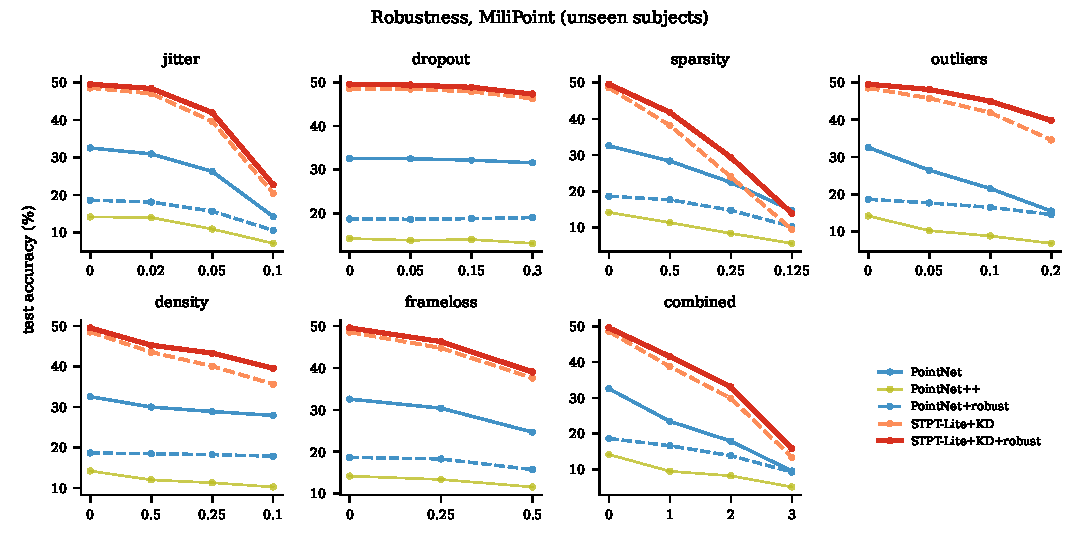
\includegraphics[width=\textwidth]{robustness_milipoint.pdf}
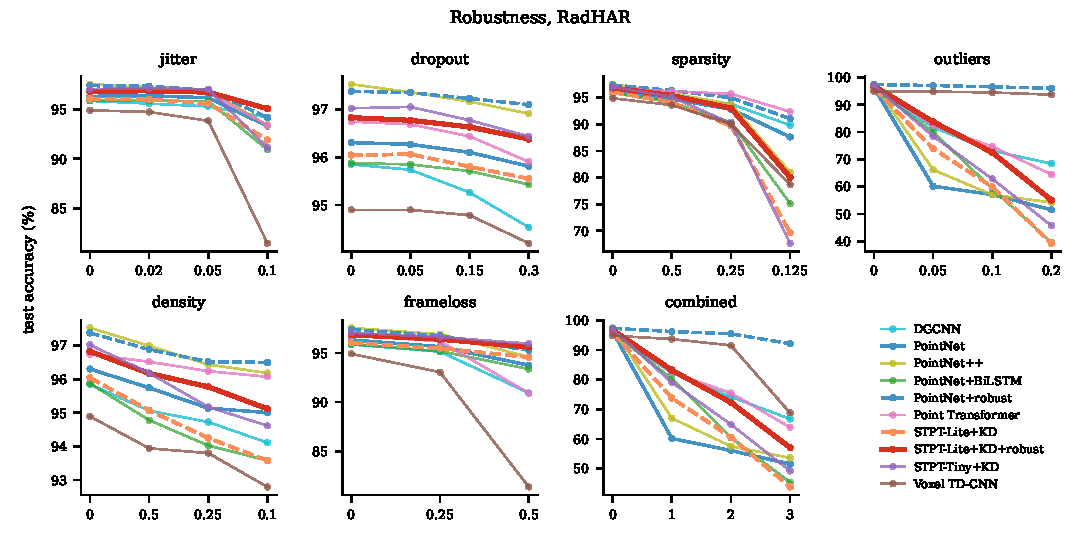
\includegraphics[width=\textwidth]{robustness_radhar.pdf}
\caption{Accuracy under controlled perturbations (identical perturbed test samples for every model). Top: MiliPoint; bottom: RadHAR.}
\label{fig:robreport}
\end{figure}
\begin{table}[h]
\centering
\caption{Robustness on MiliPoint (unseen subjects): test accuracy (\%) / prediction stability (\% of predictions unchanged w.r.t.\ clean), mean over seeds.}
\label{tab:robmilipoint}
\resizebox{\textwidth}{!}{%
\begin{tabular}{lccccc}
\toprule
Condition (level) & PointNet & PointNet+rob. & PointNet++ & STPT+KD & STPT+KD+rob. \\
\midrule
clean (0) & 32.6 / 100 & 18.7 / 100 & 14.2 / 100 & 48.5 / 100 & 49.6 / 100 \\
jitter (0.05) & 26.3 / 62 & 15.7 / 66 & 11.0 / 31 & 39.6 / 69 & 42.0 / 74 \\
dropout (0.3) & 31.6 / 73 & 19.0 / 69 & 13.1 / 53 & 46.3 / 77 & 47.3 / 80 \\
sparsity (0.25) & 22.5 / 35 & 14.8 / 29 & 8.4 / 20 & 24.0 / 29 & 29.4 / 38 \\
outliers (0.1) & 21.6 / 42 & 16.5 / 63 & 8.8 / 21 & 41.9 / 70 & 45.0 / 77 \\
density (0.25) & 28.9 / 57 & 18.2 / 50 & 11.3 / 38 & 40.1 / 58 & 43.3 / 64 \\
frameloss (0.5) & 24.7 / 44 & 15.8 / 38 & 11.6 / 30 & 37.6 / 59 & 39.0 / 61 \\
combined (2) & 17.9 / 30 & 13.8 / 36 & 8.2 / 14 & 29.9 / 44 & 33.0 / 51 \\
\bottomrule
\end{tabular}}
\end{table}
\begin{table}[h]
\centering
\caption{Robustness on RadHAR: test accuracy (\%) / prediction stability (\% of predictions unchanged w.r.t.\ clean), mean over seeds.}
\label{tab:robradhar}
\resizebox{\textwidth}{!}{%
\begin{tabular}{lccccc}
\toprule
Condition (level) & PointNet & PointNet+rob. & PointNet++ & STPT+KD & STPT+KD+rob. \\
\midrule
clean (0) & 96.3 / 100 & 97.4 / 100 & 97.5 / 100 & 96.0 / 100 & 96.8 / 100 \\
jitter (0.05) & 96.2 / 98 & 96.9 / 99 & 97.0 / 99 & 95.6 / 99 & 96.7 / 99 \\
dropout (0.3) & 95.8 / 99 & 97.1 / 99 & 96.9 / 99 & 95.5 / 99 & 96.4 / 99 \\
sparsity (0.25) & 92.8 / 96 & 95.0 / 97 & 93.8 / 96 & 89.7 / 92 & 93.0 / 95 \\
outliers (0.1) & 57.1 / 56 & 96.6 / 99 & 57.0 / 57 & 59.9 / 60 & 72.5 / 72 \\
density (0.25) & 95.1 / 98 & 96.5 / 99 & 96.4 / 98 & 94.2 / 98 & 95.8 / 98 \\
frameloss (0.5) & 93.7 / 96 & 95.2 / 97 & 94.6 / 96 & 94.6 / 97 & 95.6 / 98 \\
combined (2) & 56.0 / 55 & 95.5 / 98 & 57.5 / 57 & 60.5 / 61 & 72.3 / 72 \\
\bottomrule
\end{tabular}}
\end{table}

Fig.~\ref{fig:robust} reports test accuracy under seven perturbation types,
three severities each, applied with fixed seeds so that every model sees the
same perturbed windows. \textbf{MiliPoint (unseen people).} The proposed model
stays the most accurate under every condition except the most extreme
sparsity. Noise-robust training improves STPT-Lite+KD under all perturbations,
by 0.9--5.4 points (e.g.\ 20\% false detections: 34.6$\rightarrow$39.8\%; density
0.1: 35.6$\rightarrow$39.6\%), including jitter, which was not used in training
(22.8 vs.\ 20.5\% at $\sigma=10$\,cm). At 12.5\% of the returns kept (about one
point per frame), STPT-Lite (13.9\%) falls to the level of PointNet (14.7\%): with
almost no points per segment, intra-segment attention has nothing to attend to.
\textbf{RadHAR.} Dropout, density changes and jitter up to 5\,cm cost every
point-based model at most 2.5 points. Losing half of the segments costs DGCNN and
Point Transformer about five points but the proposed model only 1.2 points
(96.8$\rightarrow$95.6\%), which matches the even temporal attention in
Section~\ref{sec:xai}. Two conditions separate the
models. Under extreme sparsity, Point Transformer (92.4\%) and PointNet with
robust training (91.1\%) degrade least, the proposed model reaches 80.0\%, and
STPT-Lite+KD without robust training drops to 69.7\%. False detections are the
main weakness of the STPT family on RadHAR: at 20\% injected outliers the
proposed model keeps 55.1\% (39.3\% without robust training), whereas PointNet
with the same robust training keeps 96.0\% and the voxel CNN-LSTM 93.7\%.
A likely cause is that outliers corrupt the motion descriptor (centroid, mean Doppler) and receive
attention weight, while a max-pooled PointNet with robust training learns to
ignore isolated points and voxel occupancy dilutes them. Robust training
therefore helps, but it does not close this gap. A robust centroid (median) in
the motion descriptor and outlier-aware attention are the obvious next steps.


\section{Explainability}
\begin{figure}[h]
\centering
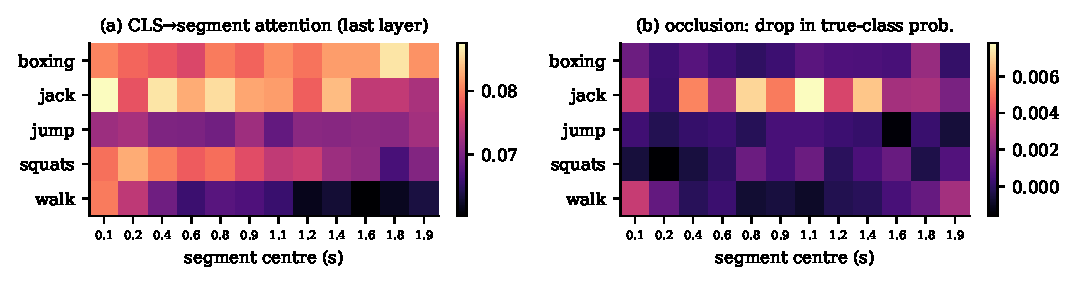
\includegraphics[width=\textwidth]{xai_temporal.pdf}
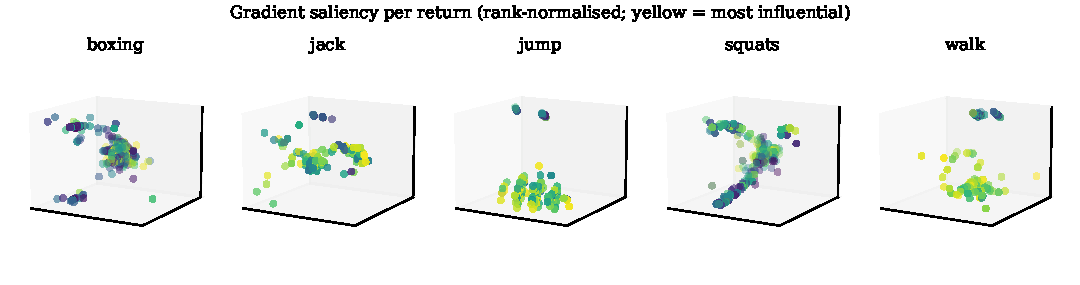
\includegraphics[width=\textwidth]{xai_saliency.pdf}
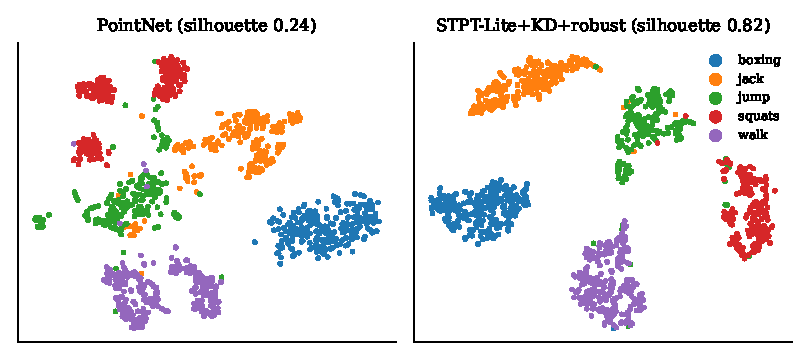
\includegraphics[width=0.75\textwidth]{tsne.pdf}
\caption{Temporal attention vs.\ occlusion importance, per-point gradient saliency, and t-SNE of embeddings (RadHAR test).}
\label{fig:xaireport}
\end{figure}
\textbf{Temporal attention and occlusion.} The [CLS] attention of the last
block is spread almost evenly over the twelve segments (0.07--0.09 per
segment, against 0.083 for uniform attention), with class-specific emphasis: the
middle of the window for jumping jacks, early segments for squats, and the
first segment for walking (Fig.~\ref{fig:xai}). Removing a single segment
(occlusion) lowers the true-class probability by less than one percentage point
on average. The model therefore integrates evidence over the whole window and
does not depend on any single 170-ms segment, which is consistent with its
tolerance to frame loss. Attention and occlusion importance agree only
moderately (Pearson $r=\xaiCorr$ over the class$\times$segment cells), so we
treat attention as a coarse indication and not as a faithful explanation.
\textbf{Point saliency.} Gradient saliency concentrates on the returns of the
moving limbs and torso and is low on isolated returns far from the body,
i.e.\ on the residual clutter that survives gating. \textbf{Embeddings.} In a
t-SNE of RadHAR test embeddings the classes form compact, well-separated
clusters (silhouette \silSTPTLiteKDrobust{} in the model's embedding space
versus \silPointNet{} for PointNet). \textbf{Errors.} The remaining RadHAR
errors are mostly windows predicted as \emph{jump} (precision 91\%), which
shares the strong vertical Doppler pattern of jumping jacks and squats. On
MiliPoint, errors concentrate in groups of kinematically similar actions.


\section{Computational efficiency}
\begin{figure}[h]
\centering
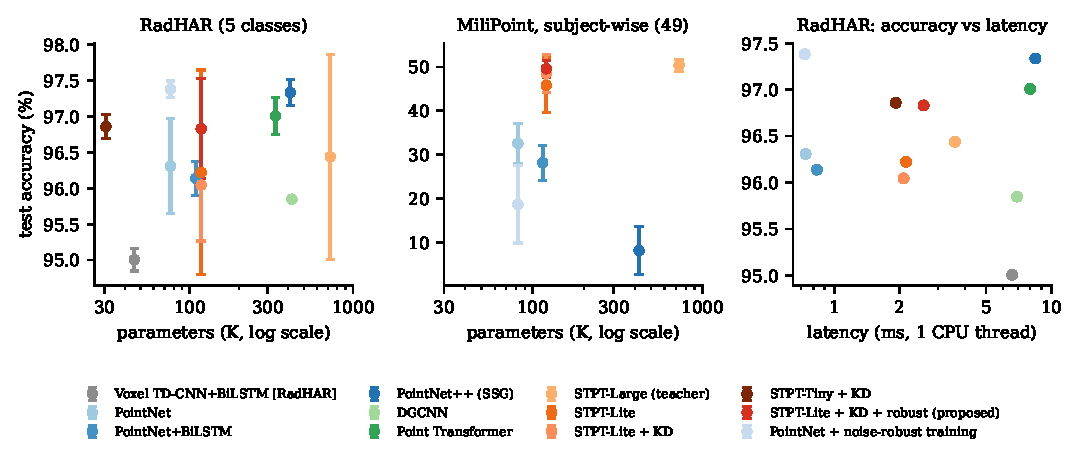
\includegraphics[width=\textwidth]{efficiency.pdf}
\caption{Accuracy vs.\ parameters and latency.}
\label{fig:effreport}
\end{figure}
STPT-Lite needs \oursMflops\,MFLOPs and \oursLat\,ms per 2-s window on one
CPU thread. It occupies \oursFpMB\,MB in FP32 and \oursIntMB\,MB with INT8
weights, and INT8 accuracy is unchanged (\rhOursIntAcc\% RadHAR,
\mpOursIntAcc\% MiliPoint).

\chapter{Working Demonstration}
\label{ch:demo}

\section{Purpose and integrity}
The demonstration (\texttt{demo/app.py}, Streamlit) executes the \emph{actual}
exported checkpoint on real radar data in the datasets' native formats. It
contains no hard-coded, random or manually assigned predictions: every number on
the screen is computed by \texttt{inference.Bundle}, which uses the same
pre-processing code as training and evaluation.

\section{How to run}
\begin{lstlisting}[numbers=none]
pip install -r requirements.txt streamlit plotly
streamlit run demo/app.py          # opens http://localhost:8501
# command-line alternative
python src/inference.py --bundle checkpoints/stpt_lite_radhar \
                        --input demo/samples/radhar_test_jump.txt
\end{lstlisting}

\section{Application structure}
\begin{description}[nosep]
\item[Sidebar] select the trained model (RadHAR or MiliPoint bundle), a bundled
  test sample (ground truth known) or an uploaded file (\texttt{.txt} RadHAR ROS
  dump, \texttt{.npz} MiliPoint frames).
\item[1 Input \& pre-processing] frame/return/window counts; 3-D view of a raw window
  with antenna returns, gated clutter and kept person returns marked; the
  pre-processed model input coloured by time.
\item[2 Recognition] recording-level prediction (majority over 2-s windows),
  ground truth if known, single-window and whole-recording latency, per-window
  class probabilities and a probability-over-time heat map. A note explains that
  softmax probabilities are not calibrated accuracy.
\item[3 Noise robustness] choose a perturbation (jitter, dropout, sparsity,
  outliers, variable density, frame loss, combined), its level and seed; the app
  shows clean vs.\ noisy point clouds, both predictions, the percentage of
  unchanged window predictions and, when ground truth is known, the window
  accuracy before and after. The test-set robustness table is shown below.
\item[4 Model \& results] parameters, FP32/INT8 size, MFLOPs, latency, held-out
  test accuracy, macro-F1/precision/recall, confusion matrix, and the full
  architecture and training configuration.
\end{description}

\section{Input validation and error handling}
Unsupported extensions, text without RadHAR point records, npz files without
\texttt{pts}/\texttt{frame} or with wrong shapes, NaN/inf values, recordings
shorter than one 2-s window, and model/data mismatches (e.g.\ a RadHAR file with
the MiliPoint model) are rejected with a message instead of crashing the app.

\section{Bundled samples}
\texttt{demo/samples/} contains 12-s excerpts of five RadHAR \emph{official test}
recordings (one per class, in the original text format) and six 4-s MiliPoint
sequences from \emph{test subjects} 8 and 9. None of them was used for training
or model selection.

\section{Screenshots}
\begin{figure}[h]\centering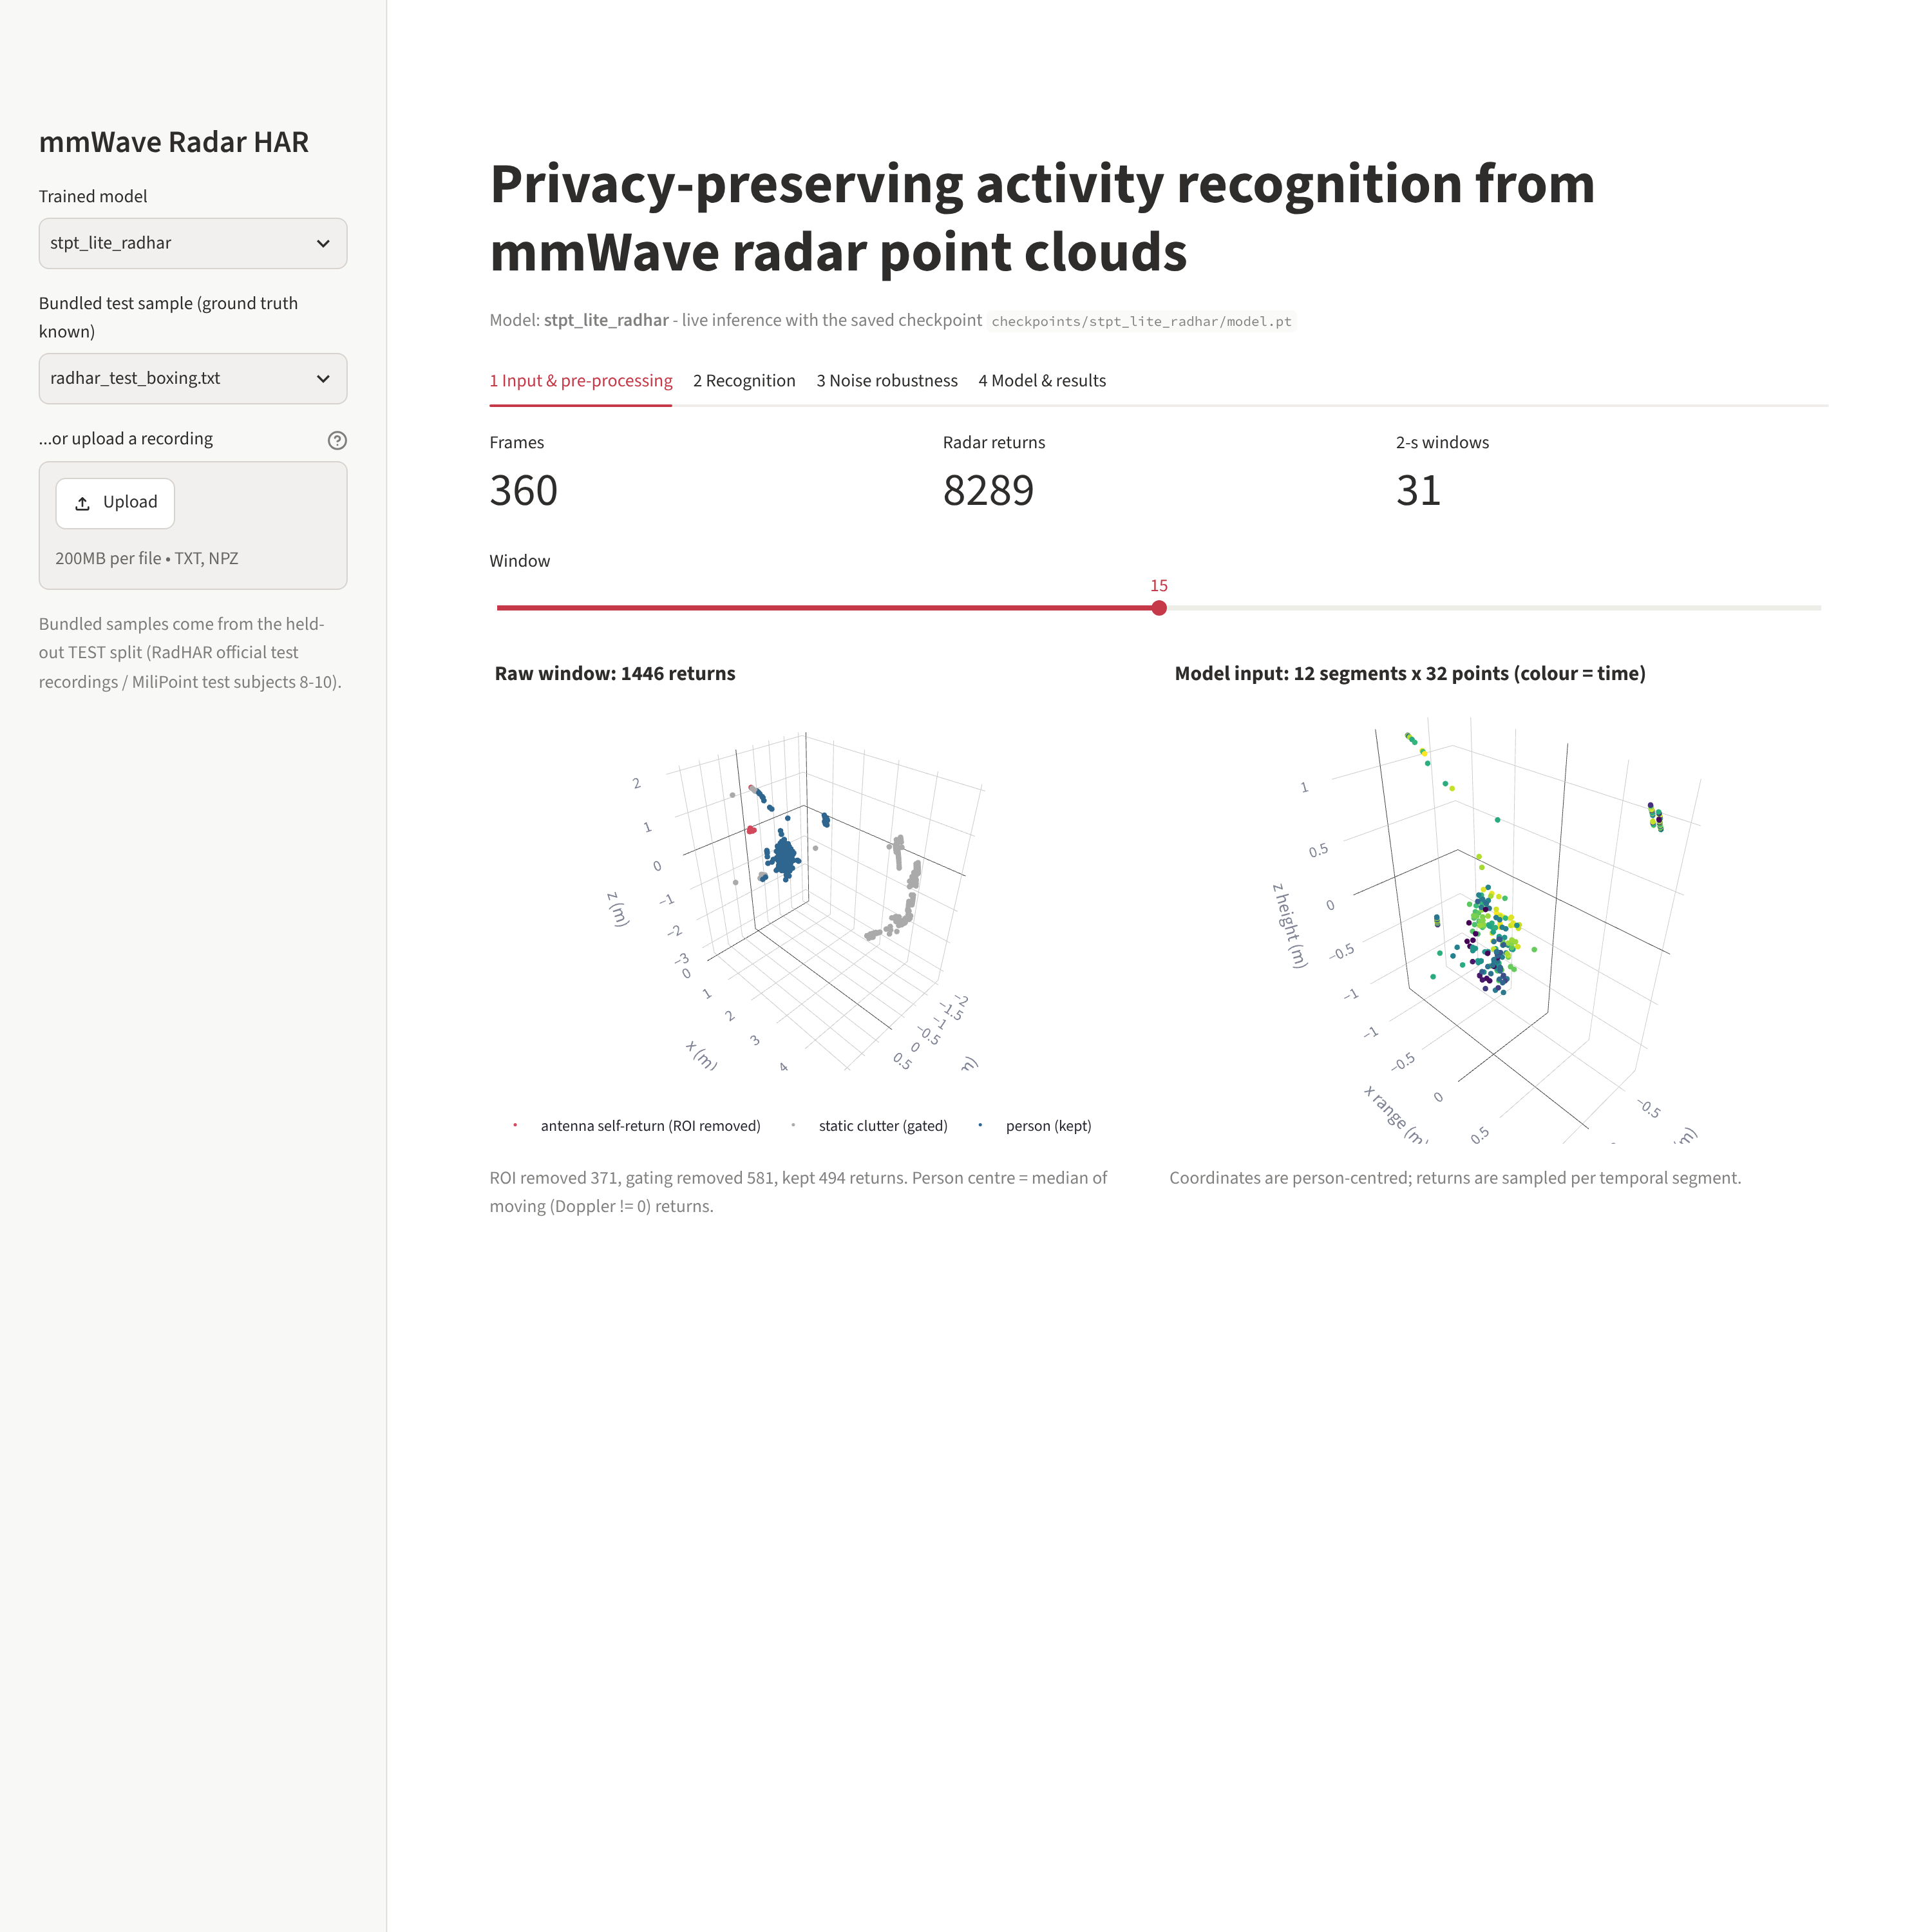
\includegraphics[width=0.92\textwidth]{demo/demo_input.png}\caption{Demonstration (real screenshot), Tab 1: raw window with antenna returns, gated clutter and kept person returns; pre-processed model input.}\label{fig:demo_input}\end{figure}
\begin{figure}[h]\centering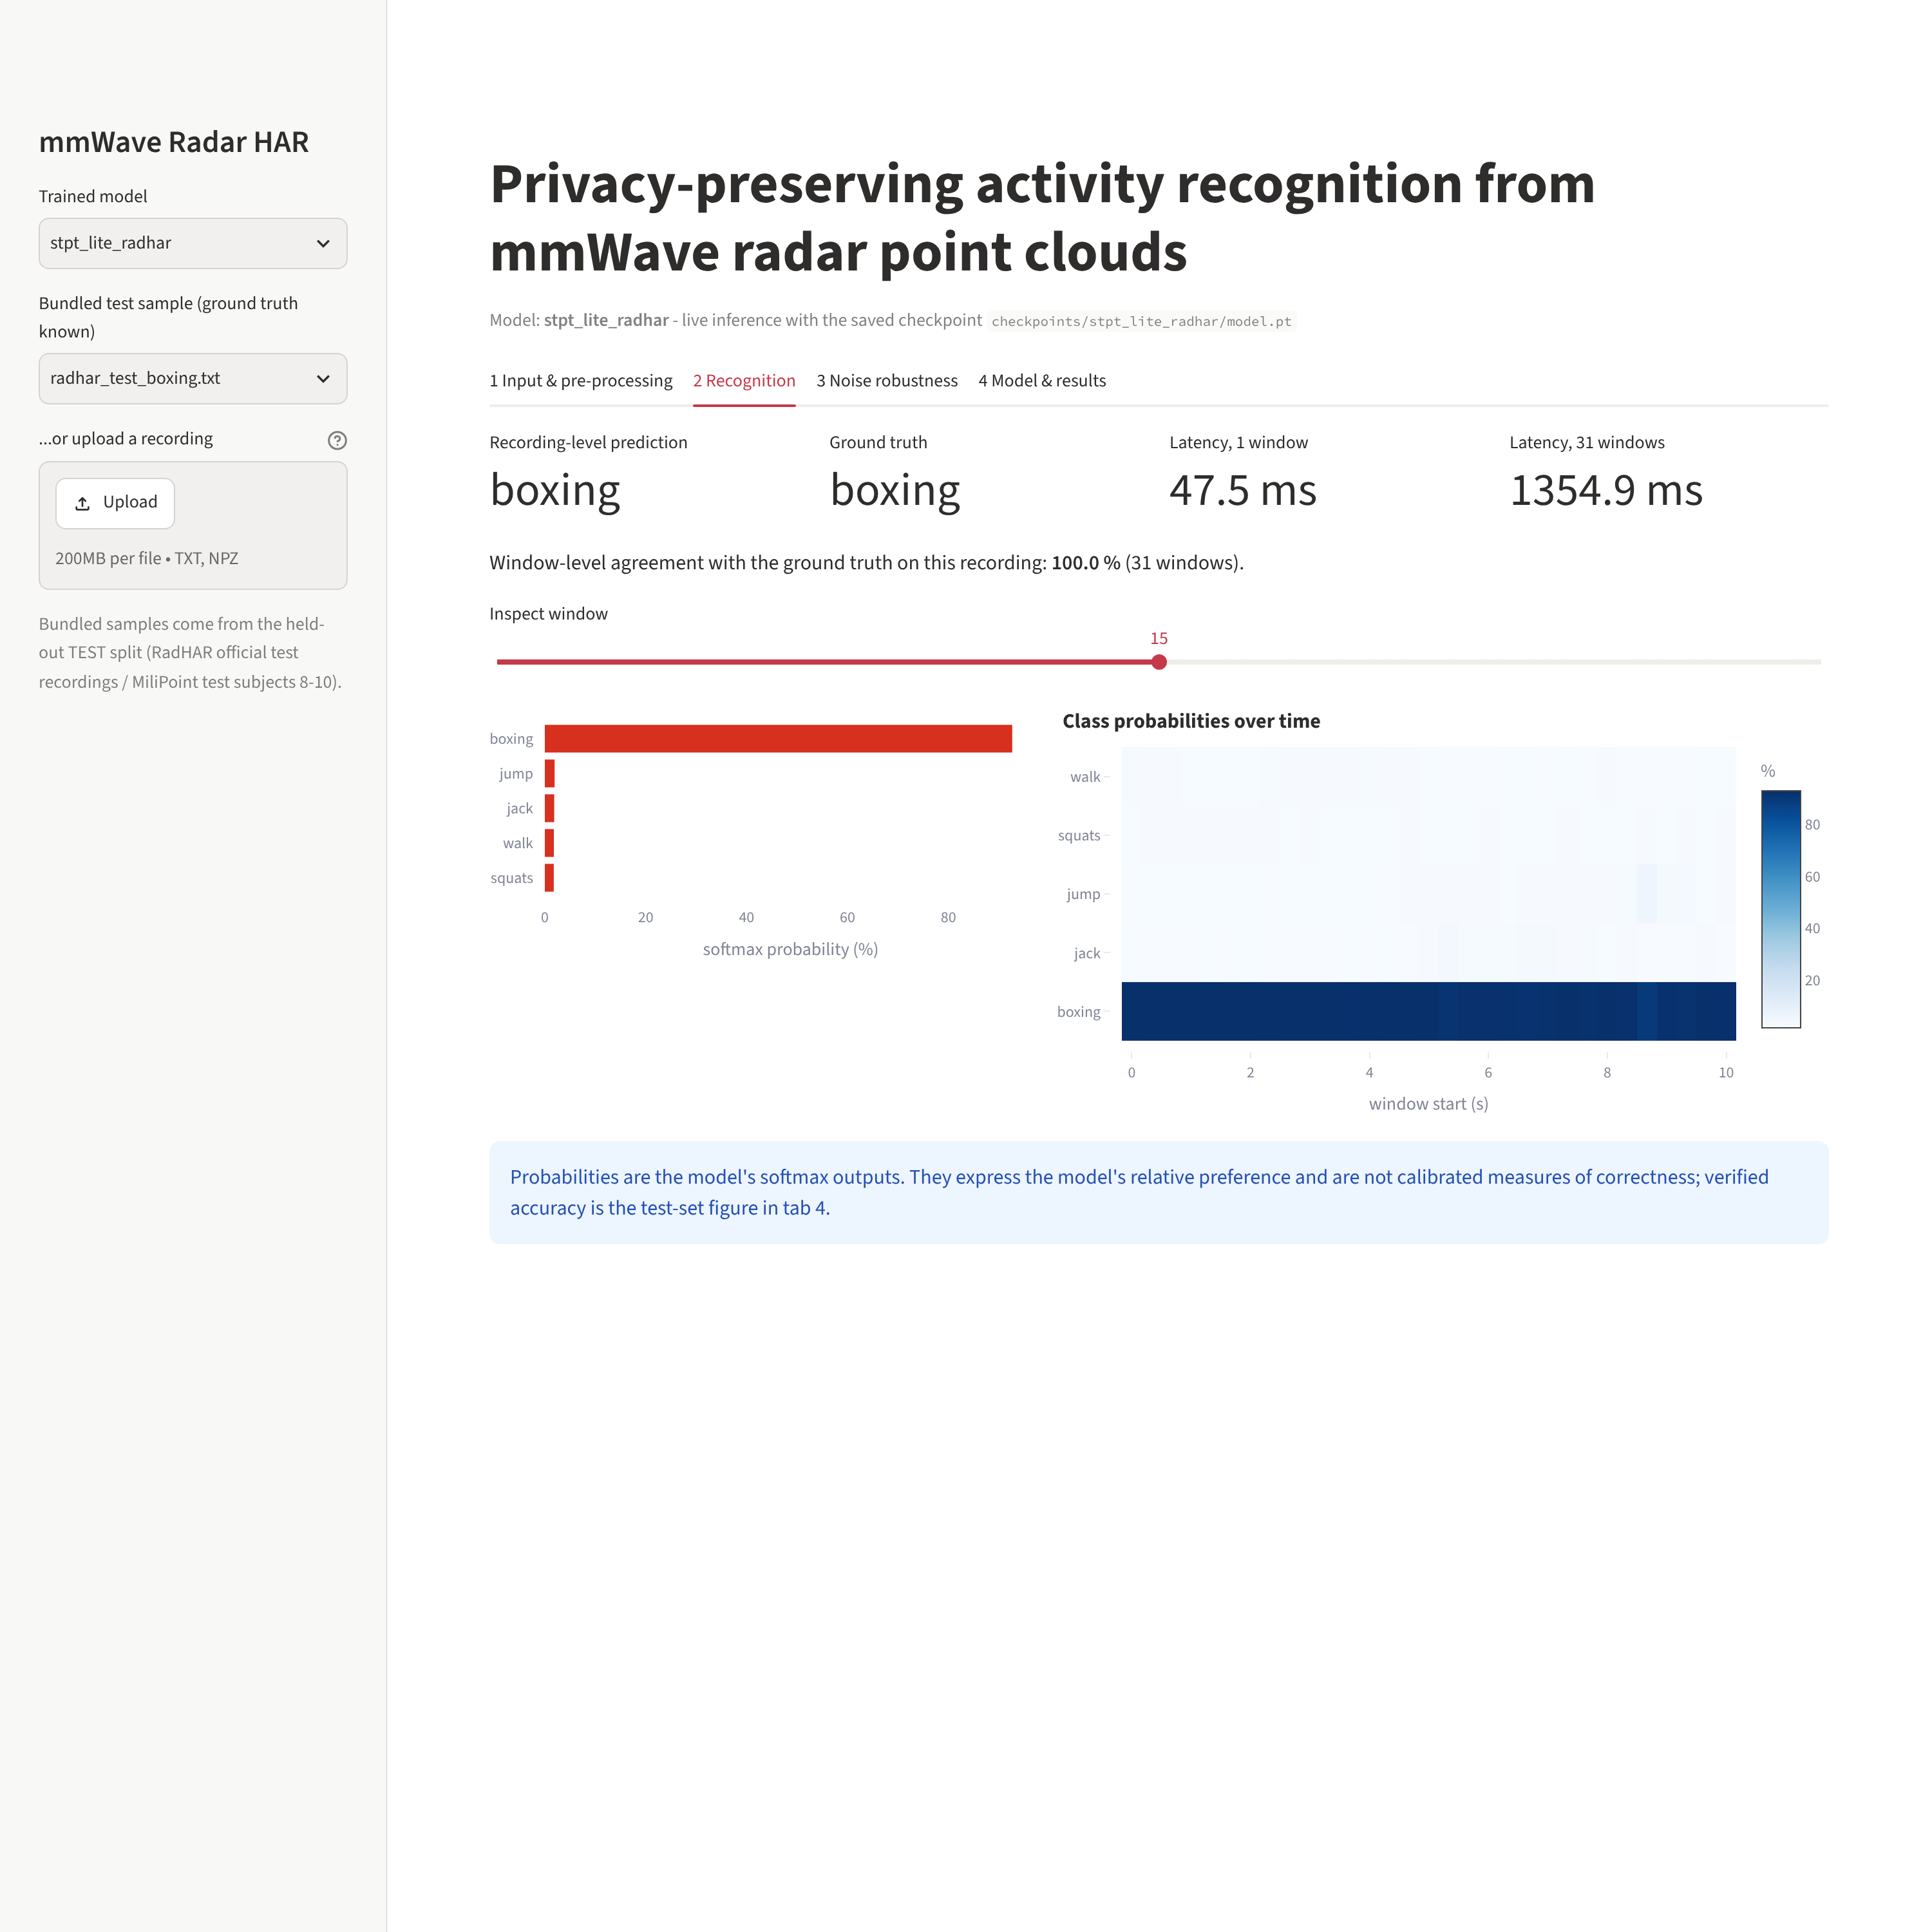
\includegraphics[width=0.92\textwidth]{demo/demo_recognition.png}\caption{Demonstration (real screenshot), Tab 2: live recording-level prediction, latency and per-window class probabilities.}\label{fig:demo_recognition}\end{figure}
\begin{figure}[h]\centering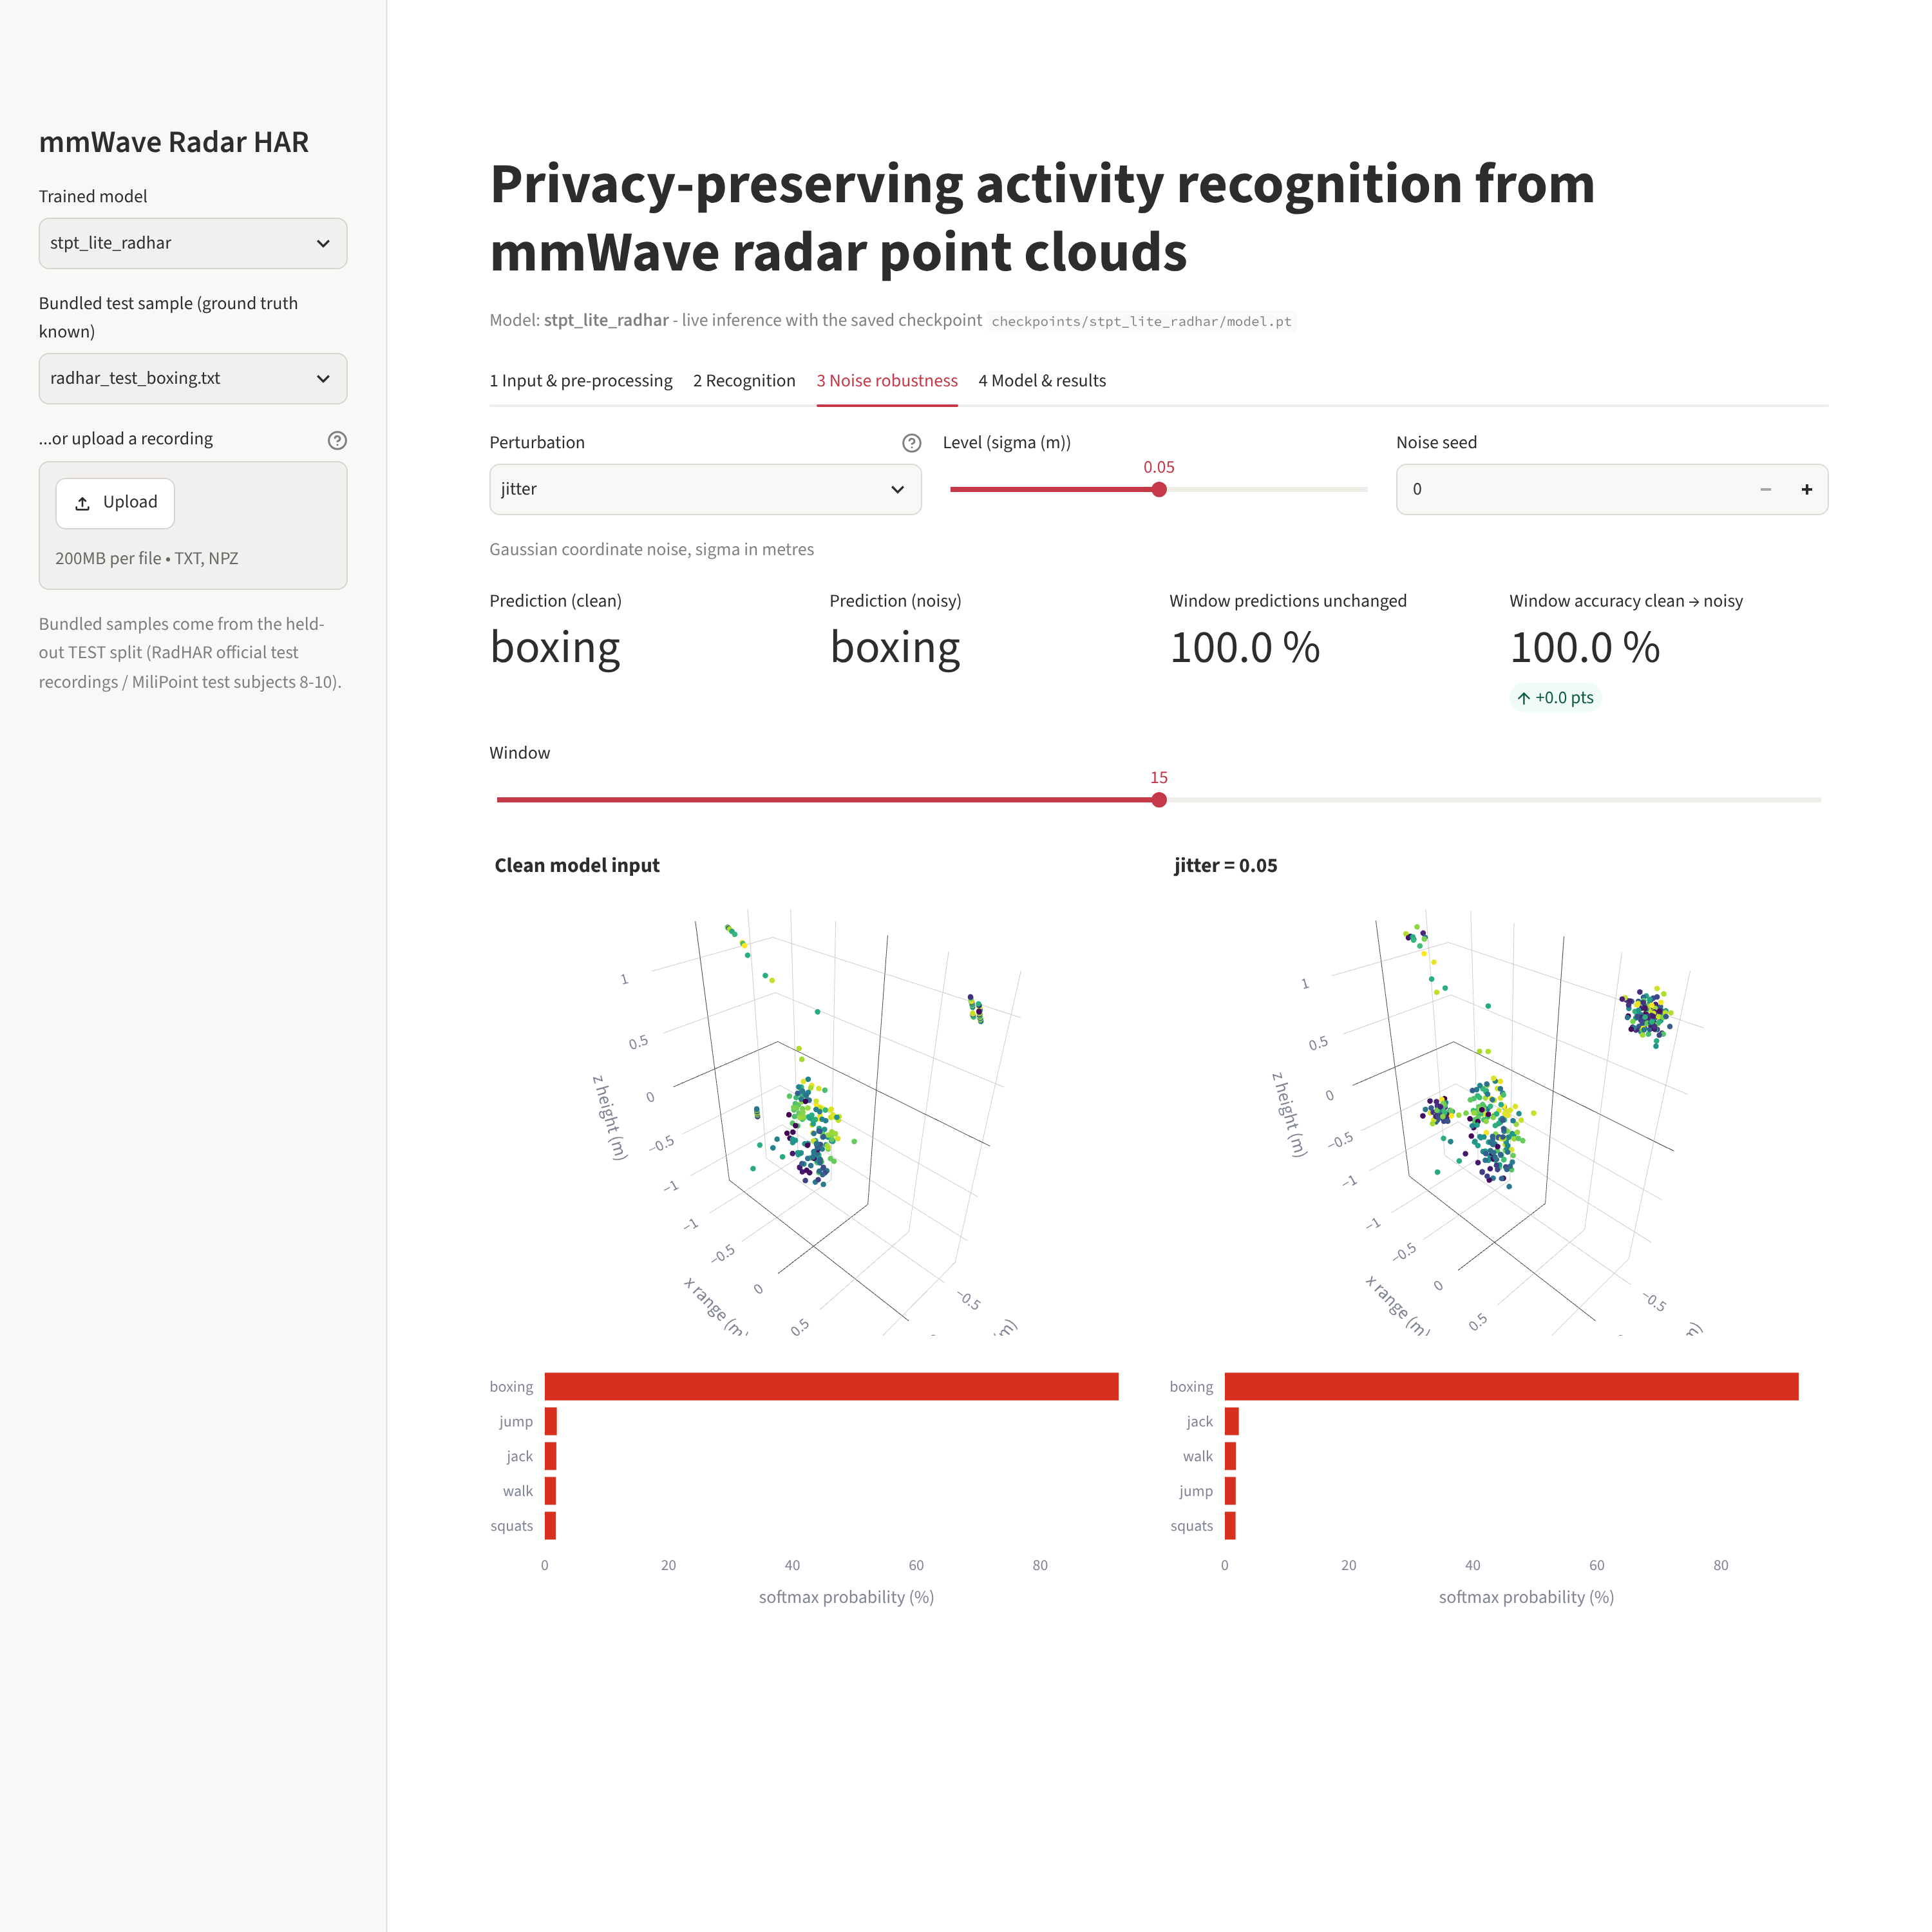
\includegraphics[width=0.92\textwidth]{demo/demo_noise.png}\caption{Demonstration (real screenshot), Tab 3: controlled noise injection; clean vs.\ noisy point cloud and predictions.}\label{fig:demo_noise}\end{figure}
\begin{figure}[h]\centering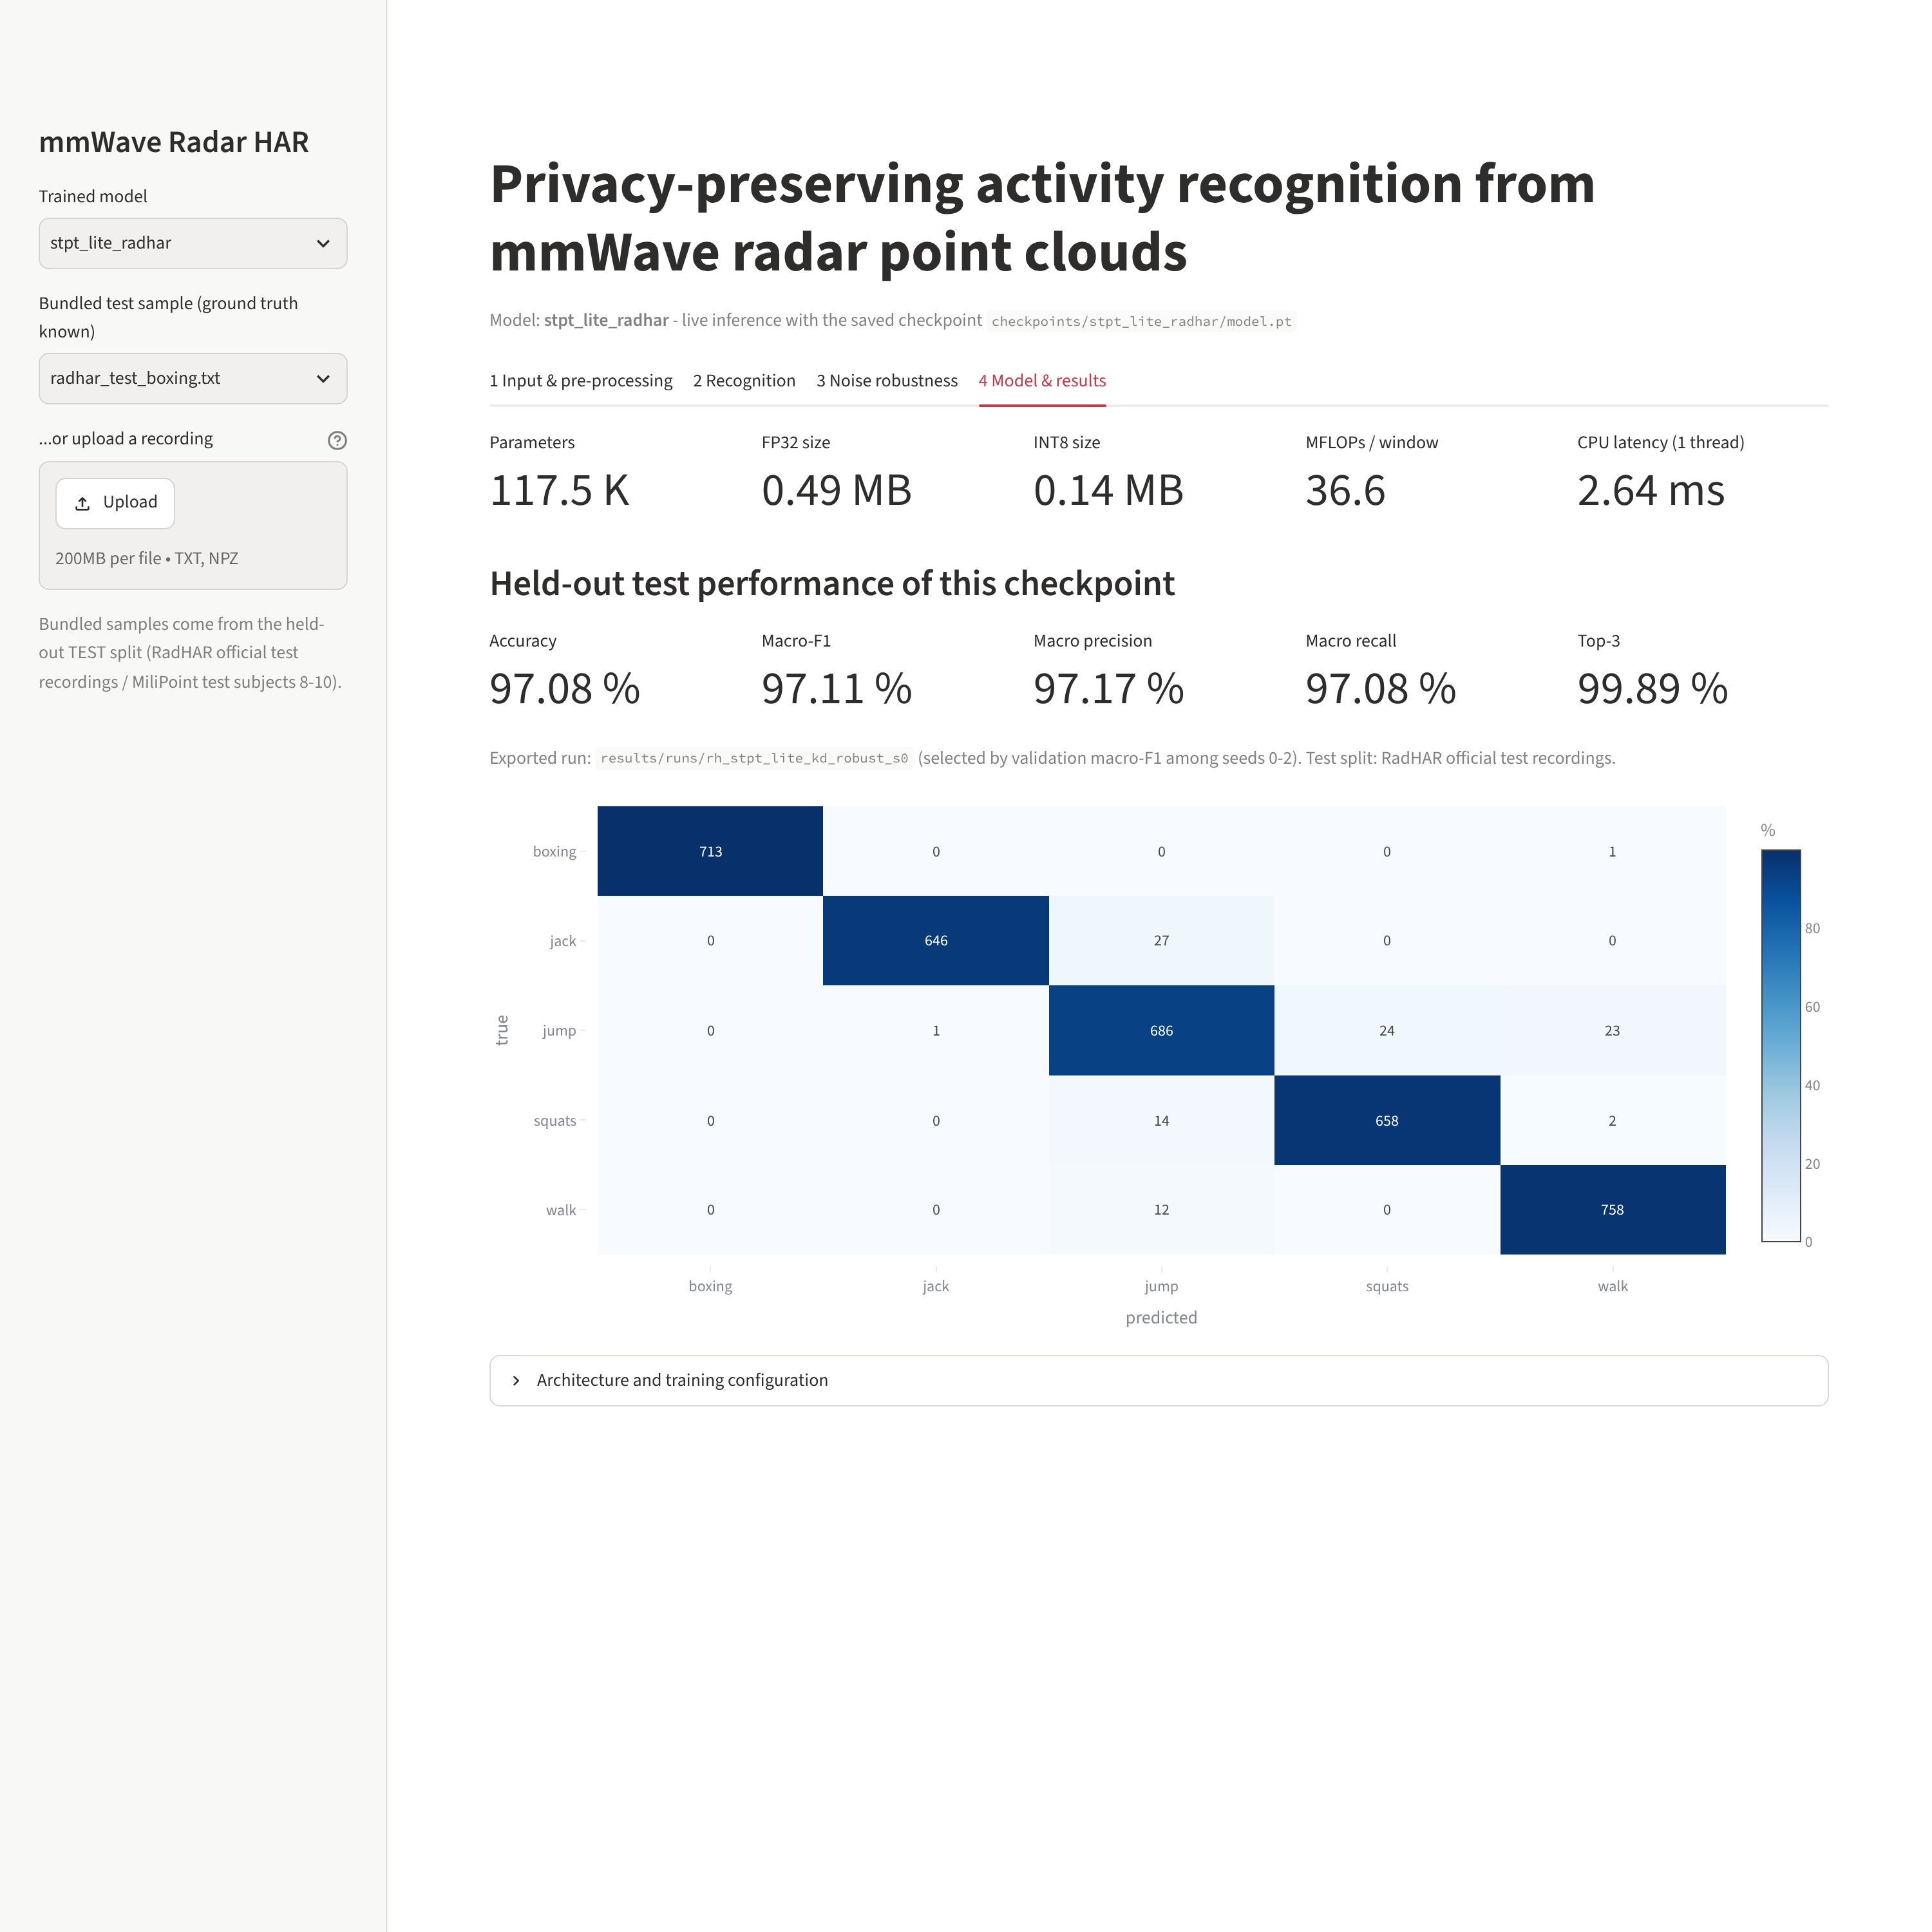
\includegraphics[width=0.92\textwidth]{demo/demo_model.png}\caption{Demonstration (real screenshot), Tab 4: model card with held-out test metrics and confusion matrix.}\label{fig:demo_model}\end{figure}

\chapter{Testing and Quality Assurance}

\section{Test strategy}
\begin{longtable}{L{2.6cm}L{6.6cm}L{4.6cm}}
\caption{Test levels.}\label{tab:testlevels}\\
\toprule
Level & What is tested & How \\
\midrule\endfirsthead
\toprule Level & What is tested & How \\ \midrule\endhead
Unit & parser on a real recording and on garbage; safe unpickler against a malicious pickle; every noise function (shape, determinism, no in-place change, effect size); every model's forward pass with empty segments & \texttt{pytest tests/} \\
Data validation & split disjointness (RadHAR recordings, MiliPoint subjects); tensor shapes and finiteness; deterministic evaluation samples; train-only statistics & \texttt{pytest} + leakage audit \\
Integration & exported bundle $\rightarrow$ raw recording $\rightarrow$ probabilities (sum to 1, deterministic); short input rejected & \texttt{pytest}, CLI \\
Checkpoint & bundle reload without retraining; seed selected by validation & CLI + demo \\
Application & app start, sample loading, preprocessing view, inference, all 7 noise conditions, sample switching, error handling & Streamlit \texttt{AppTest}, headless-browser screenshots \\
Performance & latency (median of 200, batch 1, 1 thread), FLOPs, model size & \texttt{train.py} \\
Reproducibility & identical robustness results on repeated evaluation & robustness determinism check \\
\bottomrule
\end{longtable}

\section{Results}
\begin{table}[h]
\centering
\caption{Test results (generated by \texttt{scripts/make\_qa.py}).}
\label{tab:testresults}
\begin{tabular}{lrr}
\toprule
Suite & Passed & Failed \\
\midrule
Unit / data / integration (\texttt{pytest tests/}) & 23 & 0 \\
Demo application (\texttt{scripts/apptest\_demo.py}, 28 interaction steps) & 28 & 0 \\
Leakage audit checks (\texttt{scripts/leakage\_audit.py}) & 9 & 0 \\
\bottomrule
\end{tabular}
\end{table}
The demo test drives the real application headlessly: it loads both exported models, every bundled test sample and every perturbation condition, and fails on any exception or error message shown to the user.

\section{Quality-assurance matrix}
\begin{longtable}{L{2.5cm}L{5.6cm}L{4.4cm}L{1.4cm}}
\caption{Final quality-assurance matrix (evidence-based).}\label{tab:qa}\\
\toprule
Area & Check & Evidence & Status \\
\midrule\endfirsthead
\toprule Area & Check & Evidence & Status \\ \midrule\endhead
\csname @@input\endcsname ../paper/generated/qa_rows.tex 
\bottomrule
\end{longtable}

\chapter{Limitations and Future Enhancements}

\section{Limitations}
\begin{enumerate}[nosep]
\item \textbf{RadHAR is not a subject- or session-independent benchmark.} It has
  two subjects, no subject IDs, and test recordings made minutes after training
  recordings in the same room (Chapter~\ref{ch:leak}). High RadHAR accuracy
  therefore shows generalisation to new recordings, not to new people or rooms.
\item \textbf{MiliPoint}: the radar provides $xyz$ only, action names are not
  published, and the test set has three subjects, so per-subject variance is
  large and only partly captured.
\item \textbf{Synthetic perturbations}: the robustness study perturbs recorded
  point clouds; it does not simulate the physical radar (multipath geometry,
  interference, different mounting heights or rooms).
\item \textbf{Compute}: all experiments ran on a 2-core CPU. Training was capped
  at 15 epochs with early stopping and a 20/24-frame training stride. DGCNN and
  Point Transformer on MiliPoint were run with one seed because of their cost.
  The voxel baseline uses fewer filters than the original RadHAR network.
\item \textbf{Edge claims}: latency was measured on a desktop-class CPU thread and
  storage is computed for INT8 weights; deployment on a micro-controller was not
  carried out.
\item \textbf{Scope}: no fall detection (no labels), single person only, fixed 2-s
  windows, no clinical validation.
\item \textbf{Explainability}: attention maps are not explanations in a causal
  sense \cite{jain2019attention}; occlusion and gradient saliency give
  complementary but approximate views.
\end{enumerate}

\section{Future enhancements}
\begin{enumerate}[nosep]
\item Collect or adopt a dataset with subject IDs, several rooms and fall events;
  evaluate leave-one-subject-out and cross-room.
\item Port the model to an embedded runtime (e.g.\ ONNX Runtime Mobile or an
  MCU inference library) and measure on the radar's companion processor.
\item Physics-based radar simulation for robustness (multipath, occlusion).
\item Self-supervised pre-training on unlabelled radar data (both datasets
  contain many unlabelled frames), and continuous (streaming) recognition.
\end{enumerate}

\chapter{Conclusion}

\textbf{What was developed.} A complete, reproducible pipeline for
privacy-preserving activity recognition from mmWave radar point clouds. It
comprises safe dataset loaders for RadHAR and MiliPoint, radar-specific
pre-processing (antenna-return ROI, Doppler-based person centring, 1.2\,m clutter
gating), seven model families including the proposed STPT-Lite, a seeded
noise-perturbation module, an automated leakage audit, a training/evaluation
harness with statistics, an exported inference bundle, a command-line inference
tool and an interactive Streamlit demonstration.

\textbf{Why these methods.} Every choice traces back to a measurement
(Table~\ref{tab:trace}). The clutter removal follows from the range/Doppler
analysis. The factorised attention follows from the extreme per-frame sparsity
together with strong temporal structure. Recording- and subject-disjoint splits
follow from the overlap of windows. The validation cap and the longer MiliPoint
schedule follow from observed failures (Chapter~10).

\textbf{What was demonstrated.} On 49 MiliPoint actions performed by unseen
people, the proposed STPT-Lite+KD+robust reaches \mistptlitekdrobustAcc\% top-1
(distillation alone: \mistptlitekdAcc\%), about 17 points above the best re-implemented
baseline, with \oursParamsK\,K parameters, \oursMflops\,MFLOPs, \oursLat\,ms CPU
latency and \oursIntMB\,MB of INT8 weights. Noise-robust training improves
accuracy under every perturbation type on MiliPoint without lowering clean
accuracy. On RadHAR all models saturate at about 95--98\%. Pre-training on
MiliPoint raises RadHAR accuracy with 10\% of the training recordings from
\trrhxyzscratchfTen\% to \trrhxyzmpinitfTen\%. On unseen people, removing the
intra-segment attention or the temporal Transformer costs several points.

\textbf{What was verified.} Split disjointness, absence of duplicated
recordings and frames, train-only statistics and validation-only checkpoint
selection (automated audit). The tests pass, the saved model reloads and runs on
raw files, and the demo works end to end (application test harness and
real-browser screenshots).

\textbf{What remains unresolved.} RadHAR cannot test new users or rooms. Our
PointNet++ re-implementation under-performs on MiliPoint. Under extreme
sparsity STPT-Lite falls to PointNet level, and on RadHAR it is much more
sensitive to injected false detections than PointNet with robust training. No on-device deployment or
clinical evaluation was performed (Chapter~14).


\bibliographystyle{IEEEtran}
\bibliography{../paper/refs}
\addcontentsline{toc}{chapter}{References}

\appendix
\chapter{Configuration, Installation and Commands}

\section{Default configuration (\texttt{configs/default.yaml})}
\lstinputlisting[numbers=none]{../configs/default.yaml}

\section{Installation}
\begin{lstlisting}[numbers=none]
python -m venv .venv && source .venv/bin/activate     # Windows: .venv\Scripts\activate
pip install -r requirements.txt streamlit plotly pytest
\end{lstlisting}

\section{Data preparation}
\begin{lstlisting}[numbers=none]
git clone --depth 1 https://github.com/nesl/RadHAR ext/RadHAR
git clone --depth 1 https://github.com/yizzfz/MiliPoint ext/MiliPoint
# download MiliPoint_data.zip (link in the MiliPoint README) and unzip to ext/milipoint_raw/
python src/radhar_parse.py ext/RadHAR/Data data/processed/radhar_frames.npy
python scripts/eda.py
\end{lstlisting}

\section{Training and evaluation}
\begin{lstlisting}[numbers=none]
# one run
python src/train.py --data radhar --model stpt_lite --seed 0 \
       --teacher results/runs/rh_stpt_teacher_s0 --robust 1 --tag rh_stpt_lite_kd_robust_s0
# all runs of the study (2 parallel workers)
python scripts/runner.py scripts/jobs_main.txt 2
# tables, statistics, robustness, explainability, audit
python scripts/analyze.py
python scripts/xai_robust.py robust radhar ; python scripts/xai_robust.py robust milipoint
python scripts/xai_robust.py robustfig ; python scripts/xai_robust.py xai
python scripts/leakage_audit.py ; python scripts/make_numbers.py
python -m pytest -q tests
\end{lstlisting}

\section{Inference and demonstration}
\begin{lstlisting}[numbers=none]
python scripts/export_model.py rh_stpt_lite_kd_robust checkpoints/stpt_lite_radhar radhar
python src/inference.py --bundle checkpoints/stpt_lite_radhar \
       --input demo/samples/radhar_test_walk.txt
streamlit run demo/app.py
\end{lstlisting}

\chapter{Test Log}
\begin{lstlisting}[numbers=none,basicstyle=\ttfamily\scriptsize]
.......................                                                  [100%]
==================================== PASSES ====================================
=========================== short test summary info ============================
PASSED tests/test_pipeline.py::test_parse_sample_recording
PASSED tests/test_pipeline.py::test_parse_rejects_garbage
PASSED tests/test_pipeline.py::test_safe_pickle_blocks_code
PASSED tests/test_pipeline.py::test_radhar_splits_disjoint_and_shapes
PASSED tests/test_pipeline.py::test_milipoint_subject_disjoint
PASSED tests/test_pipeline.py::test_noise_shapes_and_determinism[jitter]
PASSED tests/test_pipeline.py::test_noise_shapes_and_determinism[dropout]
PASSED tests/test_pipeline.py::test_noise_shapes_and_determinism[sparsity]
PASSED tests/test_pipeline.py::test_noise_shapes_and_determinism[outliers]
PASSED tests/test_pipeline.py::test_noise_shapes_and_determinism[density]
PASSED tests/test_pipeline.py::test_noise_shapes_and_determinism[frameloss]
PASSED tests/test_pipeline.py::test_noise_shapes_and_determinism[combined]
PASSED tests/test_pipeline.py::test_noise_effects
PASSED tests/test_pipeline.py::test_model_forward_with_empty_segments[pointnet]
PASSED tests/test_pipeline.py::test_model_forward_with_empty_segments[pointnet_lstm]
PASSED tests/test_pipeline.py::test_model_forward_with_empty_segments[pointnet2]
PASSED tests/test_pipeline.py::test_model_forward_with_empty_segments[dgcnn]
PASSED tests/test_pipeline.py::test_model_forward_with_empty_segments[pointtransformer]
PASSED tests/test_pipeline.py::test_model_forward_with_empty_segments[voxel_tdcnn]
PASSED tests/test_pipeline.py::test_model_forward_with_empty_segments[stpt_lite]
PASSED tests/test_pipeline.py::test_model_forward_with_empty_segments[stpt_tiny]
PASSED tests/test_pipeline.py::test_model_forward_with_empty_segments[stpt_teacher]
PASSED tests/test_pipeline.py::test_bundle_inference_on_real_sample
23 passed in 1.38s
\end{lstlisting}


\end{document}
